\documentclass[10pt]{article}
\usepackage[preprint]{tmlr}
\raggedbottom  % tmlr.sty sets \flushbottom, which stretches the space above paragraph headings

%%%%% NEW MATH DEFINITIONS %%%%%

\usepackage{amsmath,amsfonts,bm}

% Mark sections of captions for referring to divisions of figures
\newcommand{\figleft}{{\em (Left)}}
\newcommand{\figcenter}{{\em (Center)}}
\newcommand{\figright}{{\em (Right)}}
\newcommand{\figtop}{{\em (Top)}}
\newcommand{\figbottom}{{\em (Bottom)}}
\newcommand{\captiona}{{\em (a)}}
\newcommand{\captionb}{{\em (b)}}
\newcommand{\captionc}{{\em (c)}}
\newcommand{\captiond}{{\em (d)}}

% Highlight a newly defined term
\newcommand{\newterm}[1]{{\bf #1}}


% Figure reference, lower-case.
\def\figref#1{figure~\ref{#1}}
% Figure reference, capital. For start of sentence
\def\Figref#1{Figure~\ref{#1}}
\def\twofigref#1#2{figures \ref{#1} and \ref{#2}}
\def\quadfigref#1#2#3#4{figures \ref{#1}, \ref{#2}, \ref{#3} and \ref{#4}}
% Section reference, lower-case.
\def\secref#1{section~\ref{#1}}
% Section reference, capital.
\def\Secref#1{Section~\ref{#1}}
% Reference to two sections.
\def\twosecrefs#1#2{sections \ref{#1} and \ref{#2}}
% Reference to three sections.
\def\secrefs#1#2#3{sections \ref{#1}, \ref{#2} and \ref{#3}}
% Reference to an equation, lower-case.
\def\eqref#1{equation~\ref{#1}}
% Reference to an equation, upper case
\def\Eqref#1{Equation~\ref{#1}}
% A raw reference to an equation---avoid using if possible
\def\plaineqref#1{\ref{#1}}
% Reference to a chapter, lower-case.
\def\chapref#1{chapter~\ref{#1}}
% Reference to an equation, upper case.
\def\Chapref#1{Chapter~\ref{#1}}
% Reference to a range of chapters
\def\rangechapref#1#2{chapters\ref{#1}--\ref{#2}}
% Reference to an algorithm, lower-case.
\def\algref#1{algorithm~\ref{#1}}
% Reference to an algorithm, upper case.
\def\Algref#1{Algorithm~\ref{#1}}
\def\twoalgref#1#2{algorithms \ref{#1} and \ref{#2}}
\def\Twoalgref#1#2{Algorithms \ref{#1} and \ref{#2}}
% Reference to a part, lower case
\def\partref#1{part~\ref{#1}}
% Reference to a part, upper case
\def\Partref#1{Part~\ref{#1}}
\def\twopartref#1#2{parts \ref{#1} and \ref{#2}}

\def\ceil#1{\lceil #1 \rceil}
\def\floor#1{\lfloor #1 \rfloor}
\def\1{\bm{1}}
\newcommand{\train}{\mathcal{D}}
\newcommand{\valid}{\mathcal{D_{\mathrm{valid}}}}
\newcommand{\test}{\mathcal{D_{\mathrm{test}}}}

\def\eps{{\epsilon}}


% Random variables
\def\reta{{\textnormal{$\eta$}}}
\def\ra{{\textnormal{a}}}
\def\rb{{\textnormal{b}}}
\def\rc{{\textnormal{c}}}
\def\rd{{\textnormal{d}}}
\def\re{{\textnormal{e}}}
\def\rf{{\textnormal{f}}}
\def\rg{{\textnormal{g}}}
\def\rh{{\textnormal{h}}}
\def\ri{{\textnormal{i}}}
\def\rj{{\textnormal{j}}}
\def\rk{{\textnormal{k}}}
\def\rl{{\textnormal{l}}}
% rm is already a command, just don't name any random variables m
\def\rn{{\textnormal{n}}}
\def\ro{{\textnormal{o}}}
\def\rp{{\textnormal{p}}}
\def\rq{{\textnormal{q}}}
\def\rr{{\textnormal{r}}}
\def\rs{{\textnormal{s}}}
\def\rt{{\textnormal{t}}}
\def\ru{{\textnormal{u}}}
\def\rv{{\textnormal{v}}}
\def\rw{{\textnormal{w}}}
\def\rx{{\textnormal{x}}}
\def\ry{{\textnormal{y}}}
\def\rz{{\textnormal{z}}}

% Random vectors
\def\rvepsilon{{\mathbf{\epsilon}}}
\def\rvtheta{{\mathbf{\theta}}}
\def\rva{{\mathbf{a}}}
\def\rvb{{\mathbf{b}}}
\def\rvc{{\mathbf{c}}}
\def\rvd{{\mathbf{d}}}
\def\rve{{\mathbf{e}}}
\def\rvf{{\mathbf{f}}}
\def\rvg{{\mathbf{g}}}
\def\rvh{{\mathbf{h}}}
\def\rvu{{\mathbf{i}}}
\def\rvj{{\mathbf{j}}}
\def\rvk{{\mathbf{k}}}
\def\rvl{{\mathbf{l}}}
\def\rvm{{\mathbf{m}}}
\def\rvn{{\mathbf{n}}}
\def\rvo{{\mathbf{o}}}
\def\rvp{{\mathbf{p}}}
\def\rvq{{\mathbf{q}}}
\def\rvr{{\mathbf{r}}}
\def\rvs{{\mathbf{s}}}
\def\rvt{{\mathbf{t}}}
\def\rvu{{\mathbf{u}}}
\def\rvv{{\mathbf{v}}}
\def\rvw{{\mathbf{w}}}
\def\rvx{{\mathbf{x}}}
\def\rvy{{\mathbf{y}}}
\def\rvz{{\mathbf{z}}}

% Elements of random vectors
\def\erva{{\textnormal{a}}}
\def\ervb{{\textnormal{b}}}
\def\ervc{{\textnormal{c}}}
\def\ervd{{\textnormal{d}}}
\def\erve{{\textnormal{e}}}
\def\ervf{{\textnormal{f}}}
\def\ervg{{\textnormal{g}}}
\def\ervh{{\textnormal{h}}}
\def\ervi{{\textnormal{i}}}
\def\ervj{{\textnormal{j}}}
\def\ervk{{\textnormal{k}}}
\def\ervl{{\textnormal{l}}}
\def\ervm{{\textnormal{m}}}
\def\ervn{{\textnormal{n}}}
\def\ervo{{\textnormal{o}}}
\def\ervp{{\textnormal{p}}}
\def\ervq{{\textnormal{q}}}
\def\ervr{{\textnormal{r}}}
\def\ervs{{\textnormal{s}}}
\def\ervt{{\textnormal{t}}}
\def\ervu{{\textnormal{u}}}
\def\ervv{{\textnormal{v}}}
\def\ervw{{\textnormal{w}}}
\def\ervx{{\textnormal{x}}}
\def\ervy{{\textnormal{y}}}
\def\ervz{{\textnormal{z}}}

% Random matrices
\def\rmA{{\mathbf{A}}}
\def\rmB{{\mathbf{B}}}
\def\rmC{{\mathbf{C}}}
\def\rmD{{\mathbf{D}}}
\def\rmE{{\mathbf{E}}}
\def\rmF{{\mathbf{F}}}
\def\rmG{{\mathbf{G}}}
\def\rmH{{\mathbf{H}}}
\def\rmI{{\mathbf{I}}}
\def\rmJ{{\mathbf{J}}}
\def\rmK{{\mathbf{K}}}
\def\rmL{{\mathbf{L}}}
\def\rmM{{\mathbf{M}}}
\def\rmN{{\mathbf{N}}}
\def\rmO{{\mathbf{O}}}
\def\rmP{{\mathbf{P}}}
\def\rmQ{{\mathbf{Q}}}
\def\rmR{{\mathbf{R}}}
\def\rmS{{\mathbf{S}}}
\def\rmT{{\mathbf{T}}}
\def\rmU{{\mathbf{U}}}
\def\rmV{{\mathbf{V}}}
\def\rmW{{\mathbf{W}}}
\def\rmX{{\mathbf{X}}}
\def\rmY{{\mathbf{Y}}}
\def\rmZ{{\mathbf{Z}}}

% Elements of random matrices
\def\ermA{{\textnormal{A}}}
\def\ermB{{\textnormal{B}}}
\def\ermC{{\textnormal{C}}}
\def\ermD{{\textnormal{D}}}
\def\ermE{{\textnormal{E}}}
\def\ermF{{\textnormal{F}}}
\def\ermG{{\textnormal{G}}}
\def\ermH{{\textnormal{H}}}
\def\ermI{{\textnormal{I}}}
\def\ermJ{{\textnormal{J}}}
\def\ermK{{\textnormal{K}}}
\def\ermL{{\textnormal{L}}}
\def\ermM{{\textnormal{M}}}
\def\ermN{{\textnormal{N}}}
\def\ermO{{\textnormal{O}}}
\def\ermP{{\textnormal{P}}}
\def\ermQ{{\textnormal{Q}}}
\def\ermR{{\textnormal{R}}}
\def\ermS{{\textnormal{S}}}
\def\ermT{{\textnormal{T}}}
\def\ermU{{\textnormal{U}}}
\def\ermV{{\textnormal{V}}}
\def\ermW{{\textnormal{W}}}
\def\ermX{{\textnormal{X}}}
\def\ermY{{\textnormal{Y}}}
\def\ermZ{{\textnormal{Z}}}

% Vectors
\def\vzero{{\bm{0}}}
\def\vone{{\bm{1}}}
\def\vmu{{\bm{\mu}}}
\def\vtheta{{\bm{\theta}}}
\def\va{{\bm{a}}}
\def\vb{{\bm{b}}}
\def\vc{{\bm{c}}}
\def\vd{{\bm{d}}}
\def\ve{{\bm{e}}}
\def\vf{{\bm{f}}}
\def\vg{{\bm{g}}}
\def\vh{{\bm{h}}}
\def\vi{{\bm{i}}}
\def\vj{{\bm{j}}}
\def\vk{{\bm{k}}}
\def\vl{{\bm{l}}}
\def\vm{{\bm{m}}}
\def\vn{{\bm{n}}}
\def\vo{{\bm{o}}}
\def\vp{{\bm{p}}}
\def\vq{{\bm{q}}}
\def\vr{{\bm{r}}}
\def\vs{{\bm{s}}}
\def\vt{{\bm{t}}}
\def\vu{{\bm{u}}}
\def\vv{{\bm{v}}}
\def\vw{{\bm{w}}}
\def\vx{{\bm{x}}}
\def\vy{{\bm{y}}}
\def\vz{{\bm{z}}}

% Elements of vectors
\def\evalpha{{\alpha}}
\def\evbeta{{\beta}}
\def\evepsilon{{\epsilon}}
\def\evlambda{{\lambda}}
\def\evomega{{\omega}}
\def\evmu{{\mu}}
\def\evpsi{{\psi}}
\def\evsigma{{\sigma}}
\def\evtheta{{\theta}}
\def\eva{{a}}
\def\evb{{b}}
\def\evc{{c}}
\def\evd{{d}}
\def\eve{{e}}
\def\evf{{f}}
\def\evg{{g}}
\def\evh{{h}}
\def\evi{{i}}
\def\evj{{j}}
\def\evk{{k}}
\def\evl{{l}}
\def\evm{{m}}
\def\evn{{n}}
\def\evo{{o}}
\def\evp{{p}}
\def\evq{{q}}
\def\evr{{r}}
\def\evs{{s}}
\def\evt{{t}}
\def\evu{{u}}
\def\evv{{v}}
\def\evw{{w}}
\def\evx{{x}}
\def\evy{{y}}
\def\evz{{z}}

% Matrix
\def\mA{{\bm{A}}}
\def\mB{{\bm{B}}}
\def\mC{{\bm{C}}}
\def\mD{{\bm{D}}}
\def\mE{{\bm{E}}}
\def\mF{{\bm{F}}}
\def\mG{{\bm{G}}}
\def\mH{{\bm{H}}}
\def\mI{{\bm{I}}}
\def\mJ{{\bm{J}}}
\def\mK{{\bm{K}}}
\def\mL{{\bm{L}}}
\def\mM{{\bm{M}}}
\def\mN{{\bm{N}}}
\def\mO{{\bm{O}}}
\def\mP{{\bm{P}}}
\def\mQ{{\bm{Q}}}
\def\mR{{\bm{R}}}
\def\mS{{\bm{S}}}
\def\mT{{\bm{T}}}
\def\mU{{\bm{U}}}
\def\mV{{\bm{V}}}
\def\mW{{\bm{W}}}
\def\mX{{\bm{X}}}
\def\mY{{\bm{Y}}}
\def\mZ{{\bm{Z}}}
\def\mBeta{{\bm{\beta}}}
\def\mPhi{{\bm{\Phi}}}
\def\mLambda{{\bm{\Lambda}}}
\def\mSigma{{\bm{\Sigma}}}

% Tensor
\DeclareMathAlphabet{\mathsfit}{\encodingdefault}{\sfdefault}{m}{sl}
\SetMathAlphabet{\mathsfit}{bold}{\encodingdefault}{\sfdefault}{bx}{n}
\newcommand{\tens}[1]{\bm{\mathsfit{#1}}}
\def\tA{{\tens{A}}}
\def\tB{{\tens{B}}}
\def\tC{{\tens{C}}}
\def\tD{{\tens{D}}}
\def\tE{{\tens{E}}}
\def\tF{{\tens{F}}}
\def\tG{{\tens{G}}}
\def\tH{{\tens{H}}}
\def\tI{{\tens{I}}}
\def\tJ{{\tens{J}}}
\def\tK{{\tens{K}}}
\def\tL{{\tens{L}}}
\def\tM{{\tens{M}}}
\def\tN{{\tens{N}}}
\def\tO{{\tens{O}}}
\def\tP{{\tens{P}}}
\def\tQ{{\tens{Q}}}
\def\tR{{\tens{R}}}
\def\tS{{\tens{S}}}
\def\tT{{\tens{T}}}
\def\tU{{\tens{U}}}
\def\tV{{\tens{V}}}
\def\tW{{\tens{W}}}
\def\tX{{\tens{X}}}
\def\tY{{\tens{Y}}}
\def\tZ{{\tens{Z}}}


% Graph
\def\gA{{\mathcal{A}}}
\def\gB{{\mathcal{B}}}
\def\gC{{\mathcal{C}}}
\def\gD{{\mathcal{D}}}
\def\gE{{\mathcal{E}}}
\def\gF{{\mathcal{F}}}
\def\gG{{\mathcal{G}}}
\def\gH{{\mathcal{H}}}
\def\gI{{\mathcal{I}}}
\def\gJ{{\mathcal{J}}}
\def\gK{{\mathcal{K}}}
\def\gL{{\mathcal{L}}}
\def\gM{{\mathcal{M}}}
\def\gN{{\mathcal{N}}}
\def\gO{{\mathcal{O}}}
\def\gP{{\mathcal{P}}}
\def\gQ{{\mathcal{Q}}}
\def\gR{{\mathcal{R}}}
\def\gS{{\mathcal{S}}}
\def\gT{{\mathcal{T}}}
\def\gU{{\mathcal{U}}}
\def\gV{{\mathcal{V}}}
\def\gW{{\mathcal{W}}}
\def\gX{{\mathcal{X}}}
\def\gY{{\mathcal{Y}}}
\def\gZ{{\mathcal{Z}}}

% Sets
\def\sA{{\mathbb{A}}}
\def\sB{{\mathbb{B}}}
\def\sC{{\mathbb{C}}}
\def\sD{{\mathbb{D}}}
% Don't use a set called E, because this would be the same as our symbol
% for expectation.
\def\sF{{\mathbb{F}}}
\def\sG{{\mathbb{G}}}
\def\sH{{\mathbb{H}}}
\def\sI{{\mathbb{I}}}
\def\sJ{{\mathbb{J}}}
\def\sK{{\mathbb{K}}}
\def\sL{{\mathbb{L}}}
\def\sM{{\mathbb{M}}}
\def\sN{{\mathbb{N}}}
\def\sO{{\mathbb{O}}}
\def\sP{{\mathbb{P}}}
\def\sQ{{\mathbb{Q}}}
\def\sR{{\mathbb{R}}}
\def\sS{{\mathbb{S}}}
\def\sT{{\mathbb{T}}}
\def\sU{{\mathbb{U}}}
\def\sV{{\mathbb{V}}}
\def\sW{{\mathbb{W}}}
\def\sX{{\mathbb{X}}}
\def\sY{{\mathbb{Y}}}
\def\sZ{{\mathbb{Z}}}

% Entries of a matrix
\def\emLambda{{\Lambda}}
\def\emA{{A}}
\def\emB{{B}}
\def\emC{{C}}
\def\emD{{D}}
\def\emE{{E}}
\def\emF{{F}}
\def\emG{{G}}
\def\emH{{H}}
\def\emI{{I}}
\def\emJ{{J}}
\def\emK{{K}}
\def\emL{{L}}
\def\emM{{M}}
\def\emN{{N}}
\def\emO{{O}}
\def\emP{{P}}
\def\emQ{{Q}}
\def\emR{{R}}
\def\emS{{S}}
\def\emT{{T}}
\def\emU{{U}}
\def\emV{{V}}
\def\emW{{W}}
\def\emX{{X}}
\def\emY{{Y}}
\def\emZ{{Z}}
\def\emSigma{{\Sigma}}

% entries of a tensor
% Same font as tensor, without \bm wrapper
\newcommand{\etens}[1]{\mathsfit{#1}}
\def\etLambda{{\etens{\Lambda}}}
\def\etA{{\etens{A}}}
\def\etB{{\etens{B}}}
\def\etC{{\etens{C}}}
\def\etD{{\etens{D}}}
\def\etE{{\etens{E}}}
\def\etF{{\etens{F}}}
\def\etG{{\etens{G}}}
\def\etH{{\etens{H}}}
\def\etI{{\etens{I}}}
\def\etJ{{\etens{J}}}
\def\etK{{\etens{K}}}
\def\etL{{\etens{L}}}
\def\etM{{\etens{M}}}
\def\etN{{\etens{N}}}
\def\etO{{\etens{O}}}
\def\etP{{\etens{P}}}
\def\etQ{{\etens{Q}}}
\def\etR{{\etens{R}}}
\def\etS{{\etens{S}}}
\def\etT{{\etens{T}}}
\def\etU{{\etens{U}}}
\def\etV{{\etens{V}}}
\def\etW{{\etens{W}}}
\def\etX{{\etens{X}}}
\def\etY{{\etens{Y}}}
\def\etZ{{\etens{Z}}}

% The true underlying data generating distribution
\newcommand{\pdata}{p_{\rm{data}}}
% The empirical distribution defined by the training set
\newcommand{\ptrain}{\hat{p}_{\rm{data}}}
\newcommand{\Ptrain}{\hat{P}_{\rm{data}}}
% The model distribution
\newcommand{\pmodel}{p_{\rm{model}}}
\newcommand{\Pmodel}{P_{\rm{model}}}
\newcommand{\ptildemodel}{\tilde{p}_{\rm{model}}}
% Stochastic autoencoder distributions
\newcommand{\pencode}{p_{\rm{encoder}}}
\newcommand{\pdecode}{p_{\rm{decoder}}}
\newcommand{\precons}{p_{\rm{reconstruct}}}

\newcommand{\laplace}{\mathrm{Laplace}} % Laplace distribution

\newcommand{\E}{\mathbb{E}}
\newcommand{\Ls}{\mathcal{L}}
\newcommand{\R}{\mathbb{R}}
\newcommand{\emp}{\tilde{p}}
\newcommand{\lr}{\alpha}
\newcommand{\reg}{\lambda}
\newcommand{\rect}{\mathrm{rectifier}}
\newcommand{\softmax}{\mathrm{softmax}}
\newcommand{\sigmoid}{\sigma}
\newcommand{\softplus}{\zeta}
\newcommand{\KL}{D_{\mathrm{KL}}}
\newcommand{\Var}{\mathrm{Var}}
\newcommand{\standarderror}{\mathrm{SE}}
\newcommand{\Cov}{\mathrm{Cov}}
% Wolfram Mathworld says $L^2$ is for function spaces and $\ell^2$ is for vectors
% But then they seem to use $L^2$ for vectors throughout the site, and so does
% wikipedia.
\newcommand{\normlzero}{L^0}
\newcommand{\normlone}{L^1}
\newcommand{\normltwo}{L^2}
\newcommand{\normlp}{L^p}
\newcommand{\normmax}{L^\infty}

\newcommand{\parents}{Pa} % See usage in notation.tex. Chosen to match Daphne's book.

\DeclareMathOperator*{\argmax}{arg\,max}
\DeclareMathOperator*{\argmin}{arg\,min}

\DeclareMathOperator{\sign}{sign}
\DeclareMathOperator{\Tr}{Tr}
\let\ab\allowbreak

\usepackage{hyperref}
% Consistent spacing: table captions sit above the table, figure captions below the figure, each with a fixed gap.
% With hyperref loaded, caption also makes links land at the top of the float (hypcap).
\usepackage{caption}
\usepackage{placeins}  % \FloatBarrier in the appendix
\captionsetup[table]{position=top, skip=6pt}
\captionsetup[figure]{position=bottom, skip=8pt}
\usepackage{url}
\usepackage{booktabs}
\usepackage{array}
\usepackage{makecell}
\usepackage{graphicx}
\usepackage{amsmath}
\usepackage{amssymb}
\usepackage{xcolor}

\definecolor{tdmblue}{HTML}{2A78D6}
\definecolor{shiftorange}{HTML}{EB6834}
\definecolor{inkgray}{HTML}{4A4A4A}
\definecolor{citeblue}{HTML}{1F5FAD}

% Clickable citations, cross-references and URLs, shown as coloured text instead of boxes.
\hypersetup{colorlinks=true, citecolor=citeblue, linkcolor=citeblue, urlcolor=citeblue}
% Clickable DOIs in the bibliography (tmlr.bst only \providecommand's \doi, so this definition wins).
\newcommand{\doi}[1]{doi: \href{https://doi.org/#1}{\nolinkurl{#1}}}

\newcommand{\todo}[1]{\textcolor{red}{[TODO: #1]}}

\title{Typed Decision Models under Prevalence Shift:\\Decision Training, Calibration, and Implicit Priors}

\author{\name Abdul Rahman Iqbal \email abdul.rahmanmezzi@gmail.com \\
      \addr Independent Researcher
      \AND
      \name Muhammad Fawad Nasim \email fawad.nasim@superior.edu.pk \\
      \addr Faculty of Computer Science and Information Technology\\
      The Superior University, Lahore, Pakistan
      \AND
      \name Amir Saleem \email mramir401@gmail.com \\
      \addr Independent Researcher}

\def\month{MM}
\def\year{YYYY}
\def\openreview{\url{https://openreview.net/forum?id=XXXX}}

\begin{document}

\maketitle

\begin{abstract}
Typed decision models (TDMs) return a probability over caller-defined options, and Jev is described by its vendor as
calibrated. But in deployment class frequencies change, so calibration measured on a fixed test set need not hold where
thresholds are applied. Existing evaluations leave two gaps: the gains of vendor decision training have not been
separated from those of the backbone under an identical readout, and TDMs have been tested only at the test set's class
distribution. We ask whether decision training improves a model over its own backbone, and whether a TDM's calibration
and thresholds withstand prevalence (label) shift as well as a fine-tuned classifier's. We compare three TDMs (Jev,
Tev1-4B, Nimble-9B), their base models and two trained classifiers on identical decisions from five public datasets
under simulated shift, with 35 paired tests fixed before any test was computed. First, decision training is not
uniformly beneficial: Nimble-9B, which differs from Qwen3.5-9B only by a LoRA adapter, is better calibrated on intent
tasks but 12.0 Macro-F1 points worse on financial sentiment. Second, under moderate shift Jev's expected calibration
error (ECE) and threshold risk grow significantly more than a fine-tuned DeBERTa's only on financial sentiment, by 1.7
and 2.5 percentage points; averaged over 2{,}000 shift scenarios (exploratory), the gap is at most one point on every
dataset. Third, EM prior correction with the model's mean development prediction as its prior needs no labels and lowers
Jev's ECE under shift by 2.7 and 1.8 points on the two datasets where it is highest, although labelled recalibration
lowers it far more. The three TDMs we tested are neither uniformly better than their backbones nor uniquely fragile
under shift; for calibration, their main weakness is the miscalibration they already have without shift. We release all
inputs, code and outputs.
\end{abstract}

\section{Introduction}
\label{sec:intro}

Consider a bank that routes incoming customer messages to one of a fixed set of intents and sends a message to a
human whenever the routing model is less than 90\% confident. The threshold was chosen on validation data in which,
say, one message in ten was a complaint. After a service outage, four messages in ten are complaints. The model,
the messages of each kind and the threshold are unchanged; only the class frequencies have moved. Does the model's
confidence still mean what it meant at validation time, and does the threshold still send the intended share of
messages to a human?

This question has become practical for a new class of models. Typed decision models (TDMs), also called
``System One'' models, do not generate text: given an input and a caller-defined set of options, they return a
probability distribution over the options \citep{deusser2026jev,tang2026audit}. Jev is offered as a hosted API and
is described by its vendor as calibrated; Tev1-4B and Nimble-9B are open models fine-tuned from Qwen3.5 backbones
for the same interface. A trained classifier has a training prior that label-shift corrections can use
\citep{saerens2002adjusting,lipton2018detecting}. A zero-shot model has none. The closest substitute is an
\emph{implicit prior}: the average distribution the model predicts on a development set, which requires no labels.

Existing evaluations leave two gaps. First, the benefit of vendor ``decision training'' has not been separated from the
backbone: an audit of early TDM papers calls for same-backbone ablations \citep{tang2026audit}, existing comparisons of
a vendor TDM with its backbone read the two models out differently \citep{rafe2026systemone}, and the study that does
compare identical weights fine-tunes its own models and finds gains only on some tasks \citep{li2026llmasjev}. Second, TDMs have been compared with language models and trained classifiers at a
single class distribution \citep{deusser2026jev,rafe2026systemone}, so it is not known whether their calibration and
thresholds transfer when the class frequencies change; a recent audit of 28 TDM papers lists calibration under
deployment shift as an open problem \citep{tang2026audit}. Prior adaptation without labels has been studied for language
models and vision--language models \citep{estienne2023unsupervised,han2026labelshift}, but not for TDMs against trained
classifiers under controlled shift. We are not aware of a study that combines a commercial TDM, open TDMs paired with
their own backbones, trained classifiers and controlled prevalence shift with label-free prior correction
(\hyperref[tab:coverage]{Table~\ref*{tab:coverage}}); this combination is what allows us to ask what decision training adds and whether it
survives a change in class frequencies.

We study three research questions on five public, human-labelled datasets, using identical test items and
candidate sets for every system:
\textbf{RQ1} (decision training): does vendor decision training change accuracy and calibration relative to the same
backbone?
\textbf{RQ2} (prevalence shift): under controlled prevalence shift, do a TDM's calibration error and threshold risk
change differently from those of a fine-tuned classifier?
\textbf{RQ3} (implicit-prior correction): does expectation--maximisation (EM) prior correction with the implicit
prior reduce a TDM's calibration error under shift?
Our results concern \emph{candidate-set} decisions, in which the gold label is always among 3--22 offered options, and
\emph{simulated} label shift, in which only the class frequencies change; they do not cover full-label classification
over all 150 or 64 intents, or deployment shifts that also change the text of each class (\hyperref[sec:limitations]{Section~\ref*{sec:limitations}}).
The tests and the comparison family were fixed and hashed before the final runs, and the analysis before any test was
computed (\hyperref[sec:protocol]{Section~\ref*{sec:protocol}}); the one amendment, and earlier exposures of test data
during pipeline checks (mainly the FPB test split), are listed in \hyperref[app:deviations]{Appendix~\ref*{app:deviations}}.

Our findings are as follows (\hyperref[fig:teaser]{Figure~\ref*{fig:teaser}}; all 35 tests in \hyperref[tab:alltests]{Table~\ref*{tab:alltests}}).
\begin{itemize}
  \item \textbf{Decision training is task-dependent.} Nimble-9B, which differs from Qwen3.5-9B only by a LoRA
  adapter, is better calibrated on both intent datasets but 12.0 Macro-F1~points worse on financial sentiment, where
  its calibration error is also higher (\hyperref[sec:rq1]{Section~\ref*{sec:rq1}}). Tev1-4B is never significantly worse than
  Qwen3.5-4B, and is better on five of ten tests.
  \item \textbf{Moderate prevalence shift separates Jev from a fine-tuned classifier only a little.} At a Dirichlet
  concentration of $\alpha=1$, Jev's ECE and the excess risk of its confidence threshold grow significantly
  more than DeBERTa-v3-large's (after Holm correction) only on FPB, by 1.7 and 2.5 percentage points; averaged over
  2{,}000 shift scenarios (exploratory), the difference is at most one point on every dataset and largest on TREC-6 (\hyperref[sec:rq2]{Section~\ref*{sec:rq2}}).
  \item \textbf{Implicit-prior correction helps where calibration is poor.} EM with Jev's implicit prior, which needs
  no labels, lowers Jev's ECE under shift by 2.7~points on FPB and 1.8~points on HateXplain, the two datasets where its
  unshifted ECE is highest (0.095 and 0.279), with the same sign for every prior set; on the other three datasets the
  effect is not significant after Holm correction. Recalibration on labelled development data lowers the error much
  further (\hyperref[sec:rq3]{Section~\ref*{sec:rq3}}).
  \item \textbf{Artifacts.} We release the frozen label texts, candidate sets, prompts, evaluation code and every
  per-example probability vector \todo{repository link}.
\end{itemize}
In short, decision training helps a backbone on some tasks and hurts it on others, and prevalence shift matters less
for the TDMs we tested than the calibration error they already have without shift.

\begin{figure}[t]
  \centering
  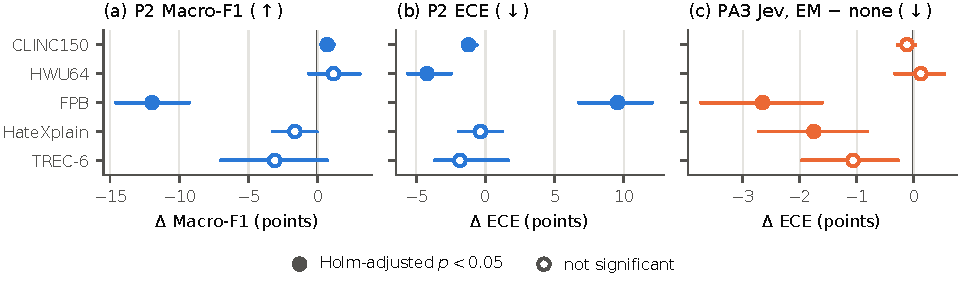
\includegraphics[width=\linewidth]{figures/fig1_teaser.pdf}
  \caption{\textbf{Decision training changes a backbone in a task-dependent direction, and label-free prior correction
  helps where calibration is poor.}
  (a, b) Paired differences between Nimble-9B and its own base model Qwen3.5-9B (same weights and 8-bit precision,
  differing only by a LoRA adapter) in Macro-F1 (higher favours Nimble) and expected calibration error (ECE; lower
  favours Nimble), in percentage points.
  (c) Change in Jev's ECE under prevalence shift ($\alpha=1$, 50 fixed target priors) when EM prior correction with
  its implicit prior is applied (lower is better).
  Bars are 95\% paired bootstrap intervals ($B=10{,}000$, unadjusted); filled markers are significant after Holm
  correction over all 35 primary tests.}
  \label{fig:teaser}
\end{figure}

\section{Related work}
\label{sec:related}

\begin{table}[t]
  \centering
  \caption{\textbf{No prior study combines vendor TDMs, matched backbones, trained classifiers and controlled prevalence
  shift with label-free prior correction.} \checkmark: covered; $\circ$: partly covered (Pair: different readouts for the
  two models, or the authors' own fine-tunes rather than a vendor TDM; Tests: intervals or tests without multiplicity
  control); --: not covered.
  Columns: TDM = commercial or vendor TDMs evaluated; Pair = TDM compared with its own backbone under the same readout;
  Trained = task-trained classifier baseline; Shift = controlled class-prior shift; Prior = label-free prior correction
  for zero-shot models; Tests = paired tests with multiplicity control.}
  \label{tab:coverage}
  \scriptsize
  \begin{tabular}{lcccccc}
    \toprule
    Study & TDM & Pair & Trained & Shift & Prior & Tests \\
    \midrule
    \citet{deusser2026jev} & \checkmark & -- & -- & -- & -- & $\circ$ \\
    \citet{rafe2026systemone} & \checkmark & $\circ$ & \checkmark & -- & -- & \checkmark \\
    \citet{li2026llmasjev} & \checkmark & $\circ$ & -- & -- & -- & $\circ$ \\
    \citet{css2026decision} & \checkmark & -- & -- & -- & -- & -- \\
    \citet{estienne2023unsupervised} & -- & -- & -- & -- & \checkmark & -- \\
    \citet{lipton2018detecting,alexandari2020maximum,garg2020unified} & -- & -- & \checkmark & \checkmark & -- & $\circ$ \\
    Our study & \checkmark & \checkmark & \checkmark & \checkmark & \checkmark & \checkmark \\
    \bottomrule
  \end{tabular}
\end{table}

\hyperref[tab:coverage]{Table~\ref*{tab:coverage}} summarises how our study relates to the closest prior work. Individually, the ingredients are
known; the question that is new is how a zero-shot decision model's calibration, thresholds and label-free prior
correction behave under prevalence shift compared with a trained classifier, and what decision training changes relative
to the identical backbone.

\paragraph{Evaluations of typed decision models.}
Jev was released in September 2026, and evaluations followed within weeks. \citet{deusser2026jev} evaluate Jev
zero-shot on 37 public datasets against two open models and report well-calibrated choice probabilities overall, with
miscalibration, mostly overconfidence, concentrated on the datasets where accuracy is low.
\citet{rafe2026systemone} compare several TDMs with trained classifiers and generative models under matched conditions
and find that the ranking depends on whether task labels exist; they also compare each decoder-based TDM, including Nimble,
with its Qwen3.5 backbone, but read the backbone out differently (by option-key likelihood), on their typed-decision
benchmark, a sample of CLINC150 and several social-science tasks. \citet{li2026llmasjev} argue that general-purpose
language models already behave like Jev-style decision models when read out by scoring the candidate labels, and that
fine-tuning helps only on some tasks. Other early studies cover annotation tasks in computational social science
\citep{css2026decision}, optimised natural-looking context that flips decisions \citep{jevout2026}, and
confidence-based escalation of LLM judges
\citep{jevjudge2026}. An audit of 28 early TDM papers finds no independent accuracy advantage of the typed readout over
comparable label-probability readouts, and lists calibration under deployment shift and the attribution of gains as
open problems \citep{tang2026audit}. All of these studies evaluate at the class distribution of the test set. Our
study varies the class distribution in a controlled way, and pairs each open TDM with its base model under the same
prompt, readout and precision, on five datasets; for Nimble-9B, which differs from its base only by an adapter, this
isolates the effect of decision training.

\paragraph{Label shift and prior correction.}
Under label (prior) shift, $p(y)$ changes while $p(x\mid y)$ stays fixed. \citet{saerens2002adjusting} re-estimate the
target prior with EM, using the classifier's posteriors and the training prior. Black-box shift estimation
\citep{lipton2018detecting} and its regularised variant \citep{azizzadenesheli2019regularized} estimate the target
prior from a confusion matrix. \citet{alexandari2020maximum} show that EM is hard to beat once the classifier is
calibrated with class-specific biases (BCTS), and \citet{garg2020unified} unify these estimators and attribute the
advantage of maximum likelihood to calibration. All of these methods assume a known source prior. For zero-shot
models, which have no training prior, prior adaptation without labels has been proposed for language models
\citep{estienne2023unsupervised}, and zero-shot CLIP models have been adapted to a given label-distribution prior
\citep{kahana2022improving} or to an unknown target distribution estimated from unlabelled test data
\citep{han2026labelshift}. We use the simplest
version of this idea, the mean predicted distribution on a development set as an implicit source prior, and test it
on a commercial TDM against a trained classifier whose source prior is known.

\paragraph{Calibration of pretrained and prompted models.}
Modern networks are often miscalibrated, and temperature scaling on held-out data is a strong fix
\citep{guo2017calibration}. Fine-tuned transformers are relatively well calibrated in-domain \citep{desai2020calibration},
whereas prompted language models carry label biases that a content-free calibration step can reduce
\citep{zhao2021calibrate}. We measure calibration with top-label ECE and selective risk \citep{geifman2017selective}, and
ask how both change when the class frequencies move.

\paragraph{Zero-shot models versus trained classifiers.}
With enough labelled data, fine-tuned encoders tend to outperform in-context or zero-shot use of larger language models
on text classification \citep{edwards2024language,bucher2024finetuned}. Fine-tuning on few examples is, however, unstable \citep{mosbach2021stability,zhang2021revisiting}, which our
training protocol takes into account. We compare against classifiers trained on the full training sets, the setting in
which a trained classifier is strongest.

\section{Setting}
\label{sec:setting}

\hyperref[fig:pipeline]{Figure~\ref*{fig:pipeline}} summarises the evaluation. Every system answers the same candidate-set decisions; prevalence
shift and recalibration are then applied to the saved probability vectors, so that all comparisons are paired.

\begin{figure}[t]
  \centering
  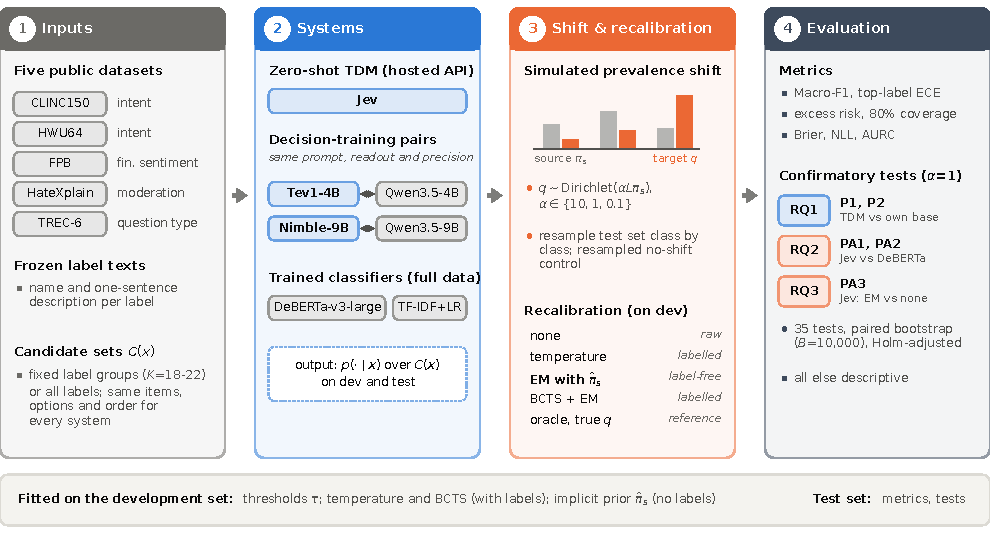
\includegraphics[width=\linewidth]{figures/fig_pipeline.pdf}
  \caption{\textbf{All systems answer identical candidate-set decisions, and shift, recalibration and tests operate on
  their saved probabilities, so every comparison is paired.}
  (1) Five public datasets with frozen label texts and fixed candidate sets. (2) A hosted TDM, two open TDMs each paired
  with its own backbone, and models trained on task labels (two classifiers on the full data and on label budgets, and a
  QLoRA adapter on Qwen3.5-4B) return a probability vector over the candidates. (3) The test set
  is resampled to simulated target priors (\hyperref[eq:shift]{Eq.~\ref*{eq:shift}}), and five recalibration arms are fitted on the unshifted
  development set (\hyperref[eq:implicit]{Eqs.~\ref*{eq:implicit}}--\nobreak\ref{eq:em}). (4) Metrics (\hyperref[eq:ece]{Eqs.~\ref*{eq:ece}} and~\ref{eq:risk}), the 35
  confirmatory tests (\hyperref[eq:pa1]{Eqs.~\ref*{eq:pa1}}--\nobreak\ref{eq:pa3}) and the label-budget curves, which are
  estimated, not tested; everything else is descriptive.}
  \label{fig:pipeline}
\end{figure}

\paragraph{Decision models and candidate sets.}
Let $\mathcal{Y}$ be the label set of a dataset and $L=|\mathcal{Y}|$ its number of classes. Each test example $x$ comes
with a candidate set $C(x)\subseteq\mathcal{Y}$ of $K$ labels that always contains the gold label. A system returns a
probability vector $p(\cdot\mid x)$ over $C(x)$. The prediction is $\hat y=\arg\max_{c\in C(x)} p(c\mid x)$, with ties
broken by candidate position, and the confidence is $\max_{c\in C(x)} p(c\mid x)$. All systems receive the same candidate
set, in the same order, for every example (\hyperref[sec:protocol]{Section~\ref*{sec:protocol}}).

\paragraph{Prevalence shift.}
Let $\pi_s$ be the class distribution of the source data and $q$ that of the deployment data. Under prevalence (label)
shift, $q\neq\pi_s$ while $p(x\mid y)$ is unchanged. We simulate it with a source-centred variant of the Dirichlet shift
of \citet{lipton2018detecting} and \citet{alexandari2020maximum}, who use a symmetric concentration, by drawing a target
prior and class counts for a sample of the test size $n$,
\begin{equation}
  q\sim\mathrm{Dirichlet}(\alpha L\,\pi_s),\qquad (n_y)_{y\in\mathcal{Y}}\mid q\sim\mathrm{Multinomial}(n,q),
  \label{eq:shift}
\end{equation}
where $\pi_s$ is the class distribution of the training split (the same for all systems), and then drawing $n_y$ test
examples of class $y$ with replacement; we call the result the shifted sample $S_q$. The concentration $\alpha L\pi_s$
centres the draws on the source prior and reduces to the usual $\mathrm{Dirichlet}(\alpha\mathbf{1})$ when $\pi_s$ is
uniform. Smaller $\alpha$ means stronger shift; we use $\alpha\in\{10,1,0.1\}$, and the confirmatory tests use $\alpha=1$.

\paragraph{Source prior and implicit prior.}
Prior correction needs the source prior $\pi_s$. For a trained classifier it is the class distribution of its training
data. A zero-shot model has no training data for the task, so we use its \emph{implicit prior}, the smoothed mean
predicted distribution over the $n_{\mathrm{dev}}$ development examples,
\begin{equation}
  \hat\pi_s(y)=\frac{\frac{1}{n_{\mathrm{dev}}}\sum_{i=1}^{n_{\mathrm{dev}}}p(y\mid x_i)+\epsilon}{1+L\epsilon},
  \qquad \epsilon=10^{-3},
  \label{eq:implicit}
\end{equation}
where $p(y\mid x_i)=0$ for $y\notin C(x_i)$; the smoothing keeps classes that the model never predicts from receiving a
prior of zero. This estimate needs no labels. It is motivated by the law of total probability: if the model's posteriors
were calibrated on the source distribution, their mean would equal the source prior, $\mathbb{E}_{x}[p(y\mid
x)]=\pi_s(y)$, and EM started from $\hat\pi_s$ would leave an unshifted sample unchanged. The implicit prior is thus the
source prior with which the model's own posteriors are consistent, a proxy in the spirit of black-box shift estimation
\citep{lipton2018detecting}. The converse does not hold. Agreement of the mean prediction with $\hat\pi_s$ is a property
of the marginal only; it does not make $p(y\mid x)$ the source posterior, which is what the likelihood argument for EM
requires \citep{saerens2002adjusting}. For a miscalibrated model, EM with $\hat\pi_s$ is therefore not a consistent
estimator of the target prior, and we treat it as an empirical, label-free correction whose effect is tested (PA3)
rather than guaranteed. A simulation with deliberately distorted posteriors (exploratory;
\hyperref[tab:emmiscal]{Table~\ref*{tab:emmiscal}}) shows the estimate degrading as calibration worsens, most for
underconfident posteriors, while staying far closer to the target prior than no correction, and with distorted
posteriors the implicit prior serves EM at least as well as the true source prior. EM also only rescales probabilities: a candidate to which the model assigns
probability zero keeps it after correction, so EM cannot repair the examples on which Jev gives the gold label
probability zero (below). Empirically, it is close to the true class distribution on the intent datasets and far from it
on FPB and HateXplain, where the models have a label bias: its total-variation distance to the development set's class distribution is
at most 0.033 for every zero-shot system on CLINC150, but 0.17--0.38 on FPB and 0.23--0.27 on HateXplain
(\hyperref[tab:implicitprior]{Table~\ref*{tab:implicitprior}}; \hyperref[fig:implicitprior]{Figure~\ref*{fig:implicitprior}}). We do not evaluate BBSE or RLLS themselves, because they need a confusion
matrix estimated on labelled data, whereas our question concerns correction without labels; labelled recalibration is
evaluated separately (BCTS+EM).

\paragraph{Recalibration arms.}
For every system we compare five ways of producing probabilities on the shifted test set; the four deployable ones are
fitted on the unshifted development set without target labels, and the oracle uses the true target prior:
\textbf{none} (raw probabilities);
\textbf{temperature} scaling \citep{guo2017calibration};
\textbf{EM} prior correction \citep{saerens2002adjusting};
\textbf{BCTS+EM}, bias-corrected temperature scaling followed by EM \citep{alexandari2020maximum}; and
\textbf{oracle}, prior correction with the true target prior $q$ (an upper reference, not a deployable method).
EM starts from $\hat q^{(0)}=\hat\pi_s$ and alternates, for the $n$ examples of the shifted sample and $y\in C(x)$,
\begin{equation}
  \tilde p^{(t)}(y\mid x)=\frac{p(y\mid x)\,\hat q^{(t)}(y)/\hat\pi_s(y)}
  {\sum_{y'\in C(x)}p(y'\mid x)\,\hat q^{(t)}(y')/\hat\pi_s(y')},\qquad
  \hat q^{(t+1)}(y)=\frac{1}{n}\sum_{i=1}^{n}\tilde p^{(t)}(y\mid x_i),
  \label{eq:em}
\end{equation}
until $\max_y|\hat q^{(t+1)}(y)-\hat q^{(t)}(y)|<10^{-6}$ (at most 100 iterations). The oracle arm applies the E-step
once with $q$ in place of $\hat q^{(t)}$.

\paragraph{EM on candidate sets.}
For CLINC150 and HWU64 the prior lives on all $L$ classes while each posterior is restricted to its candidate set, which
is why the E-step normalises over $C(x)$ only. This is the EM of \citet{saerens2002adjusting} with the pair
$z=(x,C(x))$ as the observation in place of $x$, and it inherits that method's justification if $p(z\mid y)$ is the
same in source and target. That holds in our design: on CLINC150 and HWU64 the candidate set is the fixed group $G(y)$
of the gold label, and on the other datasets it contains every label, so in both cases $C$ is determined by $y$ and
$p(z\mid y)=p(x\mid y)\,\mathbf{1}[C=G(y)]$ is unchanged by a prior shift. The order of the options carries no
information about $y$, because the gold position is counterbalanced (\hyperref[sec:protocol]{Section~\ref*{sec:protocol}}).
Bayes' rule then gives $p_t(y\mid z)\propto p_s(y\mid z)\,q(y)/\pi_s(y)$ for $y\in C(x)$ and zero outside, the E-step of
\hyperref[eq:em]{Eq.~\ref*{eq:em}}, and the M-step is the fixed point of the likelihood of the observed $z$. Two
consequences follow. Because $C(x)$ reveals the group, EM only redistributes probability among the classes of a group:
the estimated mass of each group equals its share of the shifted sample. And the source prior must be the one with which
the posteriors $p_s(y\mid z)$ are consistent, which for a zero-shot model is its implicit prior rather than the training
prior. Our shift simulation resamples whole examples with their candidate sets, so $p(z\mid y)$ is unchanged by
construction. In a deployment, an upstream step would choose the group. If that step is a fixed function of the input,
its choices alone do not break the invariance of $p(z\mid y)$ under label shift; what fails is support: when the chosen
group excludes the gold label, the restricted posterior gives that label probability zero, and no prior correction can
recover it. A simulation with exactly calibrated posteriors (exploratory; \hyperref[tab:emsim]{Table~\ref*{tab:emsim}})
bears this out: with the gold label's group as candidate set, the EM estimate of the target prior is almost as accurate
as the sample's own class shares, and it degrades steadily as a group selector misses the gold label's group more
often.

\paragraph{Metrics.}
Our main calibration metric is top-label expected calibration error with 15 equal-width confidence bins
$B_b=[(b-1)/15,\,b/15)$, the last bin closed \citep{guo2017calibration},
\begin{equation}
  \mathrm{ECE}(S)=\sum_{b=1}^{15}\frac{|B_b|}{|S|}\,\bigl|\mathrm{acc}(B_b)-\mathrm{conf}(B_b)\bigr|,
  \label{eq:ece}
\end{equation}
where $\mathrm{acc}$ and $\mathrm{conf}$ are the accuracy and mean confidence of the examples of $S$ in a bin. Selective
prediction accepts an example if its confidence $c_i$ reaches a threshold $\tau$, chosen on the development set as the
$\lceil 0.8\,n_{\mathrm{dev}}\rceil$-th largest confidence, so that (with ties, at least) 80\% of development examples are
accepted; each recalibration arm has its own threshold. Its selective risk \citep{geifman2017selective} on a sample $S$ and, under
shift, its \emph{excess risk} relative to the unshifted test sample are
\begin{equation}
  R(S;\tau)=\frac{\sum_{i\in S}\mathbf{1}[c_i\ge\tau]\,\mathbf{1}[\hat y_i\neq y_i]}{\sum_{i\in S}\mathbf{1}[c_i\ge\tau]},
  \qquad
  \Delta R(S_q)=R(S_q;\tau)-R(T;\tau),
  \label{eq:risk}
\end{equation}
where $T$ is the unshifted test sample. We also report Macro-F1, accuracy, MCC, Brier score, negative log-likelihood
(NLL, with probabilities clipped at $10^{-12}$, since Jev returns exact zeros) and the area under the risk--coverage
curve (AURC). Jev assigns probability zero to the gold label on 0.4--7\% of test examples (most on HateXplain), so its
NLL is dominated by the clip and is reported for completeness only. Because top-label ECE is biased upward on resampled data, we also report the change in Brier score and NLL
under shift (\hyperref[tab:brier]{Tables~\ref*{tab:brier}} and~\ref{tab:nll}).

\paragraph{Test statistics.}
P1 and P2 compare a TDM with its own base model on the same test examples, $\Delta=m(\mathrm{TDM})-m(\mathrm{base})$ for
$m\in\{\text{Macro-F1},\mathrm{ECE}\}$. PA1--PA3 are defined on a fixed set of $M=50$ target priors $q_1,\dots,q_M$,
drawn once from \hyperref[eq:shift]{Eq.~\ref*{eq:shift}} at $\alpha=1$. For a test sample $T$, let $S_m$ be its shifted sample under $q_m$ and
$N_m$ a no-shift control drawn by the same resampler at $T$'s own class distribution. With $J$ for Jev and $D$ for
DeBERTa-v3-large,
\begin{align}
  \mathrm{PA1}&=\frac{1}{M}\sum_{m=1}^{M}\Bigl(\bigl[\mathrm{ECE}_J(S_m)-\mathrm{ECE}_J(N_m)\bigr]
    -\bigl[\mathrm{ECE}_D(S_m)-\mathrm{ECE}_D(N_m)\bigr]\Bigr),\label{eq:pa1}\\
  \mathrm{PA2}&=\frac{1}{M}\sum_{m=1}^{M}\Bigl(\Delta R_J(S_m)-\Delta R_D(S_m)\Bigr),\label{eq:pa2}\\
  \mathrm{PA3}&=\frac{1}{M}\sum_{m=1}^{M}\Bigl(\mathrm{ECE}^{\mathrm{EM}}_J(S_m)-\mathrm{ECE}_J(S_m)\Bigr),\label{eq:pa3}
\end{align}
where each system uses its own threshold in $\Delta R$ and $\mathrm{ECE}^{\mathrm{EM}}_J$ is computed after EM with
Jev's implicit prior. Positive PA1 and PA2 mean that Jev degrades more than DeBERTa-v3-large under shift; negative PA3
means that EM helps. PA1 subtracts a resampled control because ECE is biased upward on resampled data, whereas PA2 does
not need one because selective risk, a mean of per-example losses over the accepted examples, is nearly unbiased under
resampling. \hyperref[sec:protocol]{Section~\ref*{sec:protocol}} describes how $T$ is
resampled to obtain intervals.

\paragraph{Hypotheses.}
RQ1--RQ3 of \hyperref[sec:intro]{Section~\ref*{sec:intro}} map to the following tests, all specified before the final
test-set runs.
\textbf{H1} (RQ1): vendor decision training changes Macro-F1 or ECE relative to the base model (two-sided). The
controlled test is P2 (Nimble-9B vs Qwen3.5-9B: same base weights and precision, differing only by an adapter). P1
(Tev1-4B vs Qwen3.5-4B) is the closest available comparison, since Tev1 is a full fine-tune whose exact recipe is not
published.
\textbf{H2} (RQ2): under shift, the change in ECE (PA1, \hyperref[eq:pa1]{Eq.~\ref*{eq:pa1}}) and the excess threshold risk (PA2,
\hyperref[eq:pa2]{Eq.~\ref*{eq:pa2}}) differ between Jev and DeBERTa-v3-large (two-sided).
\textbf{H3} (RQ3): EM prior correction with Jev's implicit prior lowers Jev's ECE under shift (PA3, \hyperref[eq:pa3]{Eq.~\ref*{eq:pa3}},
tested two-sided, which is conservative for this directional hypothesis). This confirmatory test concerns plain EM on
Jev only; the other arms and systems are reported descriptively.

\paragraph{Label budgets and crossover.}
RQ4 is answered by estimation, not by a test. For a trained system $s$ with $b$ training labels and seeds
$k=1,\dots,K$, let $\Delta(b)=\frac{1}{K}\sum_{k}m(s_{b,k})-m(J)$ be the paired Macro-F1 difference to Jev on the same
test examples. Its 95\% interval comes from a bootstrap that resamples both the $K$ seeds and the test examples
($B=10{,}000$), so it covers training variation as well as test-set noise. The \emph{crossover budget} is the smallest
evaluated budget $b$ whose interval lies above zero; we report it as the interval between that budget and the one before
it, or as ``not reached'' if no budget up to the full training set qualifies. As a rough guide, we also give the budget
at which the linearly interpolated point estimate first crosses zero \citep{lescao2021howmany}.

\section{Experimental protocol}
\label{sec:protocol}

\paragraph{Datasets.}
We use five public, human-labelled English datasets that represent common decision tasks
(\hyperref[tab:datasets]{Table~\ref*{tab:datasets}}): intent classification for assistants, CLINC150 in-scope \citep{larson2019evaluation} and
HWU64 \citep{liu2019benchmarking}; financial sentiment, FPB \citep{malo2014good}; hate and offensive speech,
HateXplain \citep{mathew2021hatexplain}; and question type, TREC-6 \citep{li2002learning}. CLINC150, HateXplain and
TREC-6 use their official splits. FPB has no official split; we use a public 64/16/20 split of the 50\%-agreement subset,
following \citet{araci2019finbert}, whose 970-example test set is the one used by \citet{deusser2026jev}. For HWU64 and TREC-6, which have no official development
split, the development set is a stratified sample of the training set that follows the training class distribution.
Train and development texts that duplicate a test text after normalisation (lower-casing and removing punctuation),
and texts that occur with conflicting labels, are removed; the test sets are never changed. All raw files and processed
splits are pinned by SHA-256 hashes.

\begin{table}[t]
  \centering
  \caption{\textbf{The five datasets span intent, sentiment, moderation and question-type decisions with 3 to 150
  classes.} CLINC150 and HWU64 use fixed label groups as candidate sets ($K$ = 18--22 options); the other three use all
  labels. Train/dev/test sizes after cleaning.}
  \label{tab:datasets}
  \scriptsize
  \begin{tabular}{llrrrrr}
\toprule
Dataset & Domain & Classes & Candidates $K$ & Train & Dev & Test \\
\midrule
CLINC150 & intent (assistant) & 150 & 18--19 & 14,939 & 2,994 & 4,500 \\
HWU64 & intent (home assistant) & 64 & 21--22 & 7,871 & 1,076 & 1,076 \\
FPB & financial sentiment & 3 & 3 & 3,090 & 775 & 970 \\
HateXplain & hate / offensive speech & 3 & 3 & 15,330 & 1,921 & 1,924 \\
TREC-6 & question type & 6 & 6 & 4,869 & 498 & 500 \\
\bottomrule
\end{tabular}

\end{table}

\paragraph{Label texts and candidate sets.}
Every label has a short name and a one-sentence description, written once for all systems and frozen before any model
was run. For datasets with at most 20 labels, the candidate set contains all labels. For CLINC150 and HWU64 we
partition the labels once into fixed groups (8 groups of 18--19 and 3 groups of 21--22) by balanced $k$-means on
embeddings of the label texts, and the candidate set of an example is the group of its gold label. We chose fixed groups
because a leakage audit showed that candidate sets built around the gold label (the gold label plus its nearest
neighbours) reveal the gold label from the option list alone: a classifier that never sees the text identifies it for
97.6\% of CLINC150 and 90.2\% of HWU64 examples, against 5\% chance. With fixed groups, every member of a group receives
the same set of options. The order of the options is shuffled per example with a fixed seed, with the gold position
counterbalanced across examples, and all systems read the same candidate file.

\paragraph{Systems and inputs.}
\hyperref[tab:systems]{Table~\ref*{tab:systems}} lists the systems. Jev is queried through its hosted API, with the label names as option keys
and the label descriptions as criteria; the response's version field was \texttt{jev-1.13.0} for every call (16{,}234 in the full run and 7{,}500 in
three repeats); 465 of the 16{,}234 full-run calls (464 rate-limit responses and one timeout) succeeded after one
retry, and no call failed. Jev's API returns its probabilities rounded to two decimals; we use them as returned and renormalise over the candidates. Each open TDM and its base model receive \emph{token-identical} prompts
in the TDM's own training format: the Tev1 format for Tev1-4B and Qwen3.5-4B, and the Nimble format for Nimble-9B and
Qwen3.5-9B (checked on all 16{,}234 development and test prompts). Thinking mode is disabled. The probability vector is
the softmax ($T=1$) of the candidate letters' logits at the first answer position, computed in fp32 from the final
hidden state. The two 9B models run in 8-bit precision so that they fit on a 12\,GB GPU, and the Nimble adapter is
checked to be fully loaded before every run; the two 4B models run in bf16. Local scoring was deterministic in our check:
scoring 50 CLINC150 development examples twice gave identical probabilities for all four local models. Tev1 was trained mostly on decisions with at most
eight options, so the 18--22 options of CLINC150 and HWU64 lie outside its training distribution, and the licence of its
weights was still being finalised at the time of writing. Nimble-9B is the \texttt{original-2676} release, trained on
2{,}676 synthetic examples; we do not use the later release whose training data include public TREC questions
(\hyperref[app:runs]{Appendix~\ref*{app:runs}}).

\begin{table}[t]
  \centering
  \caption{\textbf{Each open TDM is paired with its own backbone under identical prompts, readout and precision.}
  Tev1-4B with Qwen3.5-4B (Tev1 prompt format) and Nimble-9B with Qwen3.5-9B (Nimble prompt format, identical 8-bit base
  weights). Revisions are Hugging Face commit hashes. Readout: ``letters'' is the softmax ($T=1$) over the logits of the
  candidate letters at the first answer position; the trained classifiers use a softmax over each example's candidates;
  Jev returns probabilities directly.}
  \label{tab:systems}
  \scriptsize
  \setlength{\tabcolsep}{4pt}
  \begin{tabular}{lllll}
\toprule
System & Source & Revision & Precision & Readout \\
\midrule
\textsc{Typed decision models} & & & & \\
Jev & Cloudflare API (\texttt{typesafe/jev}) & \texttt{jev-1.13.0} & API & API probabilities \\
Tev1-4B & \texttt{togethercomputer/Tev1-4B-experimental} & \texttt{0b7becf0} & bf16 & letters, Tev1 format \\
Nimble-9B & \makecell[l]{Qwen3.5-9B + LoRA \\ \texttt{bespokelabs/Bespoke-Nimble-9B}} & \makecell[l]{\texttt{fe33f82b} \\ (\texttt{original-2676})} & 8-bit & letters, Nimble format \\
\midrule
\textsc{Base LLMs} & & & & \\
Qwen3.5-4B & \texttt{Qwen/Qwen3.5-4B} & \texttt{851bf6e8} & bf16 & as Tev1-4B \\
Qwen3.5-9B & \texttt{Qwen/Qwen3.5-9B} & \texttt{c2022362} & 8-bit & as Nimble-9B \\
\midrule
\textsc{Trained classifiers} & & & & \\
DeBERTa-v3-large & fine-tuned on the full training set, 5 seeds & \texttt{64a8c8ea} & fp16 & softmax \\
TF-IDF + LR & word 1--2 grams, $C$ selected on dev & scikit-learn 1.9.1 & CPU & softmax \\
\bottomrule
\end{tabular}

\end{table}

\paragraph{Trained classifiers.}
DeBERTa-v3-large \citep{he2023debertav3} is fine-tuned on the full training set with AdamW, a learning rate selected
from $\{10^{-5}, 2\cdot10^{-5}\}$ on the development set, 10\% linear warm-up, weight decay 0.01, batch size 16, mixed
precision, maximum length 128 and 5 epochs. The best checkpoint is selected by development Macro-F1 within the candidate
sets, evaluated every 100 steps. We train five seeds; a run would count as failed if its development accuracy did not
exceed that of a majority-class predictor \citep{dodge2020finetuning,mosbach2021stability}, which did not happen. All analyses use the first
seed; the other seeds are reported in \hyperref[tab:seeds]{Table~\ref*{tab:seeds}}. The TF-IDF baseline is a logistic regression on word
uni- and bigrams with sublinear term frequency; $C$ is selected on the development set from
$\{0.1, 1, 10, 10^2, 10^3, 10^4\}$, and FPB and TREC-6 select the largest value; extending the grid to $10^5$ and
$10^6$ changes their development Macro-F1 by at most 0.2~points and their test Macro-F1 by at most 0.7~points
(exploratory check). Both classifiers' probabilities are
renormalised over each example's candidate set. Note an asymmetry: the trained classifiers use the development set both
for model selection and for recalibration, whereas the zero-shot systems use it only for recalibration and the implicit
prior.

\paragraph{Label budgets.}
For RQ4, both classifiers are also trained on stratified subsets of 100, 250, 500, 1{,}000 and 2{,}500 training
examples, and of 5{,}000 where the training set is larger (HateXplain, HWU64, CLINC150), with five subset seeds per
budget; the full training set is the last point of each curve, with all five DeBERTa-v3-large seeds. Class quotas are
proportional to the training frequencies, with at least one example per class where the budget allows it; at 100
labels, CLINC150 has examples for only 100 of its 150 classes (\hyperref[tab:shots]{Table~\ref*{tab:shots}}).
DeBERTa-v3-large uses the settings above with a fixed schedule: 20 epochs up to 500 labels and 5 epochs above, with at
least 500 optimizer steps, following the advice for few-sample fine-tuning
\citep{mosbach2021stability,zhang2021revisiting}. The learning rate, $C$ and the checkpoint are selected on the full
development set at every budget. A failed run would be restarted with one of three reserve seeds per dataset and
budget; none failed.

\paragraph{Task fine-tuning of the base model.}
Condition (b) of the decision-training comparison fine-tunes Qwen3.5-4B on the target task with QLoRA
\citep{hu2022lora,dettmers2023qlora} at 100, 500 and 2{,}500 labels, using the same subsets as above and three seeds. The
adapter has rank 16, $\alpha=32$ and dropout 0.05 on the same projection matrices as the Nimble-9B adapter; it is trained
on a 4-bit NF4 copy of the base with learning rate $10^{-4}$, effective batch size 16, the DeBERTa schedule and a
cross-entropy loss over the candidate letters at the answer position. Checkpoints are selected by development Macro-F1
every 100 steps. Every reported prediction comes from the kept adapter on the bf16 base, with the same prompt, assistant
prefix and letter readout as Qwen3.5-4B and Tev1-4B, so the three 4B conditions (a) frozen base, (b) task QLoRA and (c)
Tev1-4B differ only in their weights.

\paragraph{Statistical tests.}
The 35 confirmatory tests are P1 and P2 (Macro-F1 and ECE on five datasets each; 20 tests) and PA1--PA3 (five datasets
each; 15 tests). P1 and P2 use a paired bootstrap over test examples with $B=10{,}000$ replicates; both systems and both
metrics use the same resampled indices. For PA1--PA3 (\hyperref[eq:pa1]{Eqs.~\ref*{eq:pa1}}--\nobreak\ref{eq:pa3}), the estimand is the mean over a fixed set of 50 target priors
drawn once at $\alpha=1$ (centred on the training prior); it is therefore conditional on this set of priors, and the
intervals reflect only the finiteness of the test set. Each of $B=10{,}000$ replicates draws a class-stratified bootstrap
sample of the test set and builds all 50 shifted samples from it by resampling with replacement, so that Jev and
DeBERTa-v3-large are evaluated on identical samples. PA1 compares each shifted ECE with a no-shift control drawn by the
same resampler at the base sample's own class prior, because top-label ECE is biased upward on resampled data. PA2
compares risks, which are nearly unbiased under resampling, with the base sample itself. The point estimates of P1 and P2 are the differences on the full test set, those of
PA1--PA3 the means of the bootstrap replicates. We report percentile 95\% intervals,
which are not adjusted for multiplicity, and two-sided $p=\min\{1,\,2\min\{\Pr(\Delta\le0),\Pr(\Delta\ge0)\}\}$, adjusted with the
Holm procedure \citep{holm1979simple} over all 35 tests (also for PA3, whose hypothesis is directional). With
$B=10{,}000$, a raw $p$ of zero is reported as $p<0.0002$ $(=2/B)$, and its Holm-adjusted value as $p<0.007$
$(=35\cdot2/B)$. Quantities fitted on the development set (thresholds, implicit priors, temperatures) are held fixed
within the bootstrap, so the intervals do not include development-set uncertainty. The descriptive prevalence-shift
experiment uses 200 Dirichlet draws per $\alpha$ for all systems and all five arms, with and without replacement.

\paragraph{Protocol and runs.}
Hypotheses, tests, the comparison family, all configurations and the code were fixed and recorded as SHA-256 hashes
before the final runs, and every final run was verified against these hashes. One amendment followed three
code audits; it changed the analysis, the DeBERTa failed-run rule and the Jev error handling, but not the code used by
the local language models. It was made after the first local test predictions had been produced, but before the
DeBERTa and Jev runs and before any of the 35 tests or any shift analysis was computed on the final runs
(\hyperref[app:deviations]{Appendix~\ref*{app:deviations}}). Before the freeze, some pipeline checks were run on test
splits, mainly FPB's, including early versions of PA1--PA3 and of the shift experiment on FPB;
\hyperref[app:deviations]{Appendix~\ref*{app:deviations}} discloses them.
The local models and both trained classifiers were run on one NVIDIA RTX 4070 Ti (12\,GB); Jev, a hosted model, was
queried through its API for the main runs in about two hours, inside the protocol's 72-hour window (\hyperref[app:runs]{Appendix~\ref*{app:runs}}).
The label-budget study was specified with the rest of the protocol; its QLoRA settings, trainer and curve analysis were
fixed and hashed in a second freeze before any of its final test predictions, after a development-only pilot that left every
setting unchanged (\hyperref[app:deviations]{Appendix~\ref*{app:deviations}}). It reuses the Jev and zero-shot
predictions of the main study.

\section{Results}
\label{sec:results}

\paragraph{Validity checks.}
All 16{,}234 Jev calls and all local predictions returned a valid probability vector: no request failed after retries
and no input was refused, including on HateXplain. On the 970-example FPB test set that \citet{deusser2026jev} also use,
Jev's accuracy is 0.744, consistent with the 0.730 they report. Full-data DeBERTa-v3-large reaches 0.976 accuracy on
TREC-6, close to the 0.974 reported for fully fine-tuned RoBERTa-large \citep{gao2021making}, and 0.703 Macro-F1 on
HateXplain, slightly above the best value we found reported for that test split, 0.699 \citep{kim2022why}. The four local
models gave identical probabilities when 50 CLINC150 development examples were scored twice. Jev is not: in four runs over the same 500 test examples per dataset, it returned the same
prediction for 96.4--99.8\% of examples but the same probability vector for only 19.4--87.4\% of them, with differences of
up to 0.29 between runs; its ECE on these subsets varied by at most 0.012 between runs (\hyperref[app:results]{Appendix~\ref*{app:results}}). All
analyses use a single full run of each system.

\paragraph{Overview.}
\hyperref[tab:exp1]{Table~\ref*{tab:exp1}} gives the test-set results without shift. Full-data DeBERTa-v3-large has the highest Macro-F1 point
estimate on all five datasets, although Jev is within 0.3~points on CLINC150. Among the zero-shot systems in
\hyperref[tab:exp1]{Table~\ref*{tab:exp1}}, Jev has the highest Macro-F1 point estimate on every dataset (by 0.3~points over Qwen3.5-9B on
FPB). No zero-shot system is reliable on HateXplain (Macro-F1 at most 0.514), where even TF-IDF reaches 0.645.
Calibration varies more by task than by system class: ECE is at most 0.020 for all zero-shot systems on CLINC150, but
between 0.214 and 0.340 on HateXplain. These comparisons are descriptive; the tested comparisons follow.

\begin{table}[t]
  \centering
  \caption{\textbf{Full-data DeBERTa-v3-large has the highest Macro-F1 point estimate on every dataset, and the
  calibration of zero-shot systems depends more on the task than on the system.} Test-set Macro-F1 and ECE (15 bins,
  top label), candidate-restricted, no shift. These are point estimates; tested comparisons are in
  \hyperref[fig:pairs]{Figure~\ref*{fig:pairs}} and \hyperref[tab:pa]{Table~\ref*{tab:pa}}.}
  \label{tab:exp1}
  \scriptsize
  \setlength{\tabcolsep}{3pt}
  \begin{tabular}{lrrrrrrrrrr}
\toprule
 & \multicolumn{2}{c}{CLINC150} & \multicolumn{2}{c}{HWU64} & \multicolumn{2}{c}{FPB} & \multicolumn{2}{c}{HateXplain} & \multicolumn{2}{c}{TREC-6} \\
\cmidrule(lr){2-3} \cmidrule(lr){4-5} \cmidrule(lr){6-7} \cmidrule(lr){8-9} \cmidrule(lr){10-11}
System & F1$\uparrow$ & ECE$\downarrow$ & F1$\uparrow$ & ECE$\downarrow$ & F1$\uparrow$ & ECE$\downarrow$ & F1$\uparrow$ & ECE$\downarrow$ & F1$\uparrow$ & ECE$\downarrow$ \\
\midrule
\multicolumn{11}{l}{\textsc{Typed decision models}} \\
Jev & 0.978 & 0.007 & 0.908 & 0.036 & 0.752 & 0.095 & 0.514 & 0.279 & 0.922 & 0.042 \\
Tev1-4B & 0.964 & 0.008 & 0.895 & 0.040 & 0.735 & 0.072 & 0.458 & 0.214 & 0.889 & 0.038 \\
Nimble-9B & 0.962 & 0.008 & 0.896 & 0.035 & 0.629 & 0.263 & 0.470 & 0.336 & 0.872 & 0.043 \\
\midrule
\multicolumn{11}{l}{\textsc{Base LLMs}} \\
Qwen3.5-4B & 0.939 & 0.011 & 0.866 & 0.058 & 0.635 & 0.204 & 0.441 & 0.247 & 0.882 & 0.037 \\
Qwen3.5-9B & 0.955 & 0.020 & 0.884 & 0.078 & 0.749 & 0.168 & 0.487 & 0.340 & 0.903 & 0.061 \\
\midrule
\multicolumn{11}{l}{\textsc{Trained classifiers (full data)}} \\
DeBERTa-v3-large & 0.980 & 0.013 & 0.939 & 0.030 & 0.870 & 0.111 & 0.703 & 0.141 & 0.971 & 0.021 \\
TF-IDF + LR & 0.950 & 0.015 & 0.900 & 0.098 & 0.693 & 0.167 & 0.645 & 0.069 & 0.891 & 0.071 \\
\bottomrule
\end{tabular}

\end{table}

\subsection{RQ1: What decision training changes}
\label{sec:rq1}

\paragraph{Decision training improves the 9B backbone's calibration on intent tasks and lowers its Macro-F1 on financial
sentiment by 12~points.}
Nimble-9B differs from Qwen3.5-9B only by a LoRA adapter: the base weights, 8-bit precision, prompts and readout are
identical. On CLINC150 the adapter lowers ECE by 1.2~points (95\% CI $[-1.5,-0.6]$; Holm-adjusted $p<0.007$) and raises
Macro-F1 by 0.7~points ($[0.2, 1.2]$; $p=0.029$). On HWU64 it lowers ECE by 4.2~points ($[-5.6,-2.5]$; $p<0.007$). On FPB,
by contrast, Nimble-9B's Macro-F1 is 12.0~points below its base ($[-14.6,-9.3]$; $p<0.007$) and its ECE is 9.6~points
higher ($[6.8, 12.1]$; $p<0.007$). On HateXplain and TREC-6 neither difference is significant after correction; the
largest of these, $-3.1$ Macro-F1~points on TREC-6, has an interval of $[-7.0, 0.7]$ (\hyperref[fig:pairs]{Figure~\ref*{fig:pairs}}).

\paragraph{Tev1-4B is never significantly worse than its base model.}
Tev1-4B's Macro-F1 is higher than Qwen3.5-4B's on CLINC150 ($+2.5$, $[1.9, 3.1]$; $p<0.007$), HWU64 ($+2.8$,
$[1.1, 4.8]$; $p=0.040$) and FPB ($+10.0$, $[7.4, 12.7]$; $p<0.007$), and its ECE is lower on FPB ($-13.2$,
$[-15.7,-10.4]$; $p<0.007$) and HateXplain ($-3.2$, $[-5.2,-1.4]$; $p=0.029$). None of the ten differences favours the
base model significantly. Because Tev1 is a full fine-tune whose exact base revision and recipe are not published, and
because the 18--22 options of the intent datasets lie outside its training distribution, this pair is the closest
available comparison rather than a controlled one. On HWU64, 614 of the 1{,}076 test texts also occur in MASSIVE
\citep{fitzgerald2023massive}; on the 462 remaining examples every system, including the trained classifiers, loses 2.2
to 5.9 Macro-F1~points, the P2 calibration result holds ($-4.3$ ECE points, $[-5.8,-1.1]$), and the P1 Macro-F1
difference keeps its sign but is no longer resolved ($+3.0$, $[-0.03, 8.3]$; exploratory, \hyperref[tab:hwu64]{Table~\ref*{tab:hwu64}}).

The two pairs thus point in opposite directions on FPB: Tev1-4B scores 10.0 Macro-F1~points above its base, and
Nimble-9B 12.0~points below its own. Nimble-9B's loss is concentrated on the neutral class: it labels 285 of the 565
neutral test sentences as positive, against 159 for Qwen3.5-9B, so that its recall on neutral sentences falls from 0.64
to 0.36 while its recall on positive and negative sentences rises (0.88 to 0.96 and 0.89 to 0.95; descriptive,
\hyperref[tab:fpbconf]{Table~\ref*{tab:fpbconf}}). A later Nimble release, whose training data include public TREC questions, scores
0.963 Macro-F1 on TREC-6 against 0.872 for the release we test (exploratory; \hyperref[app:results]{Appendix~\ref*{app:results}}), which
suggests that the training data, not only decision training, affect the result.

\begin{figure}[t]
  \centering
  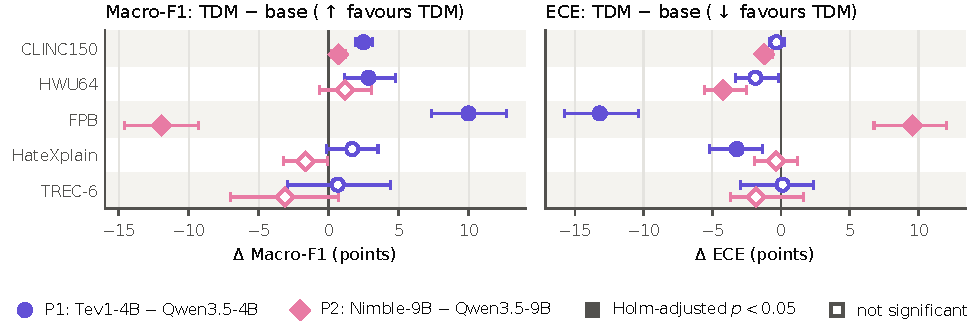
\includegraphics[width=\linewidth]{figures/fig2_pairs.pdf}
  \caption{\textbf{Tev1-4B is never significantly worse than its base model, whereas Nimble-9B is better calibrated on
  intent tasks and 12 Macro-F1~points worse on FPB.} Paired differences (TDM $-$ base) in percentage points with 95\%
  paired bootstrap intervals ($B=10{,}000$, unadjusted). Filled markers: significant after Holm correction over all 35
  primary tests.}
  \label{fig:pairs}
\end{figure}

\subsection{RQ2: Prevalence shift}
\label{sec:rq2}

\paragraph{At moderate shift, Jev and DeBERTa-v3-large are distinguishable after correction only on FPB, and the size
of that difference depends on the shift scenarios.}
On the fixed set of 50 target priors, the shift-induced change in ECE at $\alpha=1$ is 1.7~points larger for Jev than for
DeBERTa-v3-large on FPB (PA1; $[1.0, 2.5]$; $p<0.007$), and the excess risk of the 80\%-coverage threshold is 2.5~points
larger ($[1.8, 3.2]$; $p<0.007$; PA2). On the other four datasets neither difference is significant after correction
(\hyperref[tab:pa]{Table~\ref*{tab:pa}}); on CLINC150 and HWU64 the intervals lie within $\pm0.5$ points.

Because these confirmatory estimates are conditional on one set of target priors, we repeated PA1--PA3 with five other
prior sets (exploratory, added after the results were known; \hyperref[tab:pasens]{Table~\ref*{tab:pasens}}). On FPB, Jev's ECE change exceeds
DeBERTa-v3-large's for every prior set, but by 0.3 to 1.7~points (the frozen set is among the largest), and its excess
risk by 0.6 to 2.5~points (frozen set 2.5). On TREC-6, Jev's ECE change is larger by 0.8 to 1.2~points for every set. On HateXplain the
direction depends on the prior set: the frozen set favours Jev ($-0.8$), the five others favour DeBERTa-v3-large ($+0.2$
to $+0.8$). Averaged over 2{,}000 target priors drawn at $\alpha=1$ (exploratory; \hyperref[tab:papop]{Table~\ref*{tab:papop}}), the PA1
difference is $+0.4$ points on FPB, $0.0$ on HateXplain and $+1.0$ on TREC-6, and at most $0.1$ on the intent datasets;
on FPB and HateXplain the difference varies widely between single priors (standard deviation 5.4 and 7.4~points), so a
set of 50 priors is not enough to pin down its mean. PA3, in contrast, keeps its sign and remains clearly negative:
$-1.7$ points on FPB (frozen set $-2.7$) and $-2.0$ on HateXplain (frozen set $-1.8$). We therefore read RQ2 as follows: under moderate shift, Jev's calibration error grows by at most 1.7~points more than that of a fine-tuned classifier on any prior set, and by at most one point on average over shifts;
the direction is consistent on FPB and TREC-6, and the size of such differences depends on which shifts are considered. Two facts call for caution about the significant FPB results (PA1 and PA2). FPB is the
dataset whose test split was used in pipeline checks before the protocol was frozen (\hyperref[app:deviations]{Appendix~\ref*{app:deviations}}),
and the size of the estimate is not stable across prior sets (0.3 to 1.7~points). Jev's own run-to-run variation in ECE
on FPB, measured on repeated calls over 500 test examples, is at most 0.6~points (\hyperref[tab:jevrepeat]{Table~\ref*{tab:jevrepeat}}), well below
the frozen estimate, so the non-determinism of the API is unlikely to explain the FPB result, whereas its size depends
strongly on the prior set. We therefore do not treat RQ2 as evidence that Jev is more fragile under shift than a trained classifier; the
robust conclusion is that the difference is small.

\begin{table}[t]
  \centering
  \caption{\textbf{The EM correction effect (PA3) is stable across shift scenarios, whereas the Jev--DeBERTa difference
  (PA1, PA2) varies in size, and on HateXplain in sign.} Frozen: the confirmatory estimate on the pre-specified set of 50
  target priors ($B=10{,}000$; $\dagger$: Holm-adjusted $p<0.05$). Exploratory: range of the estimates over five other sets
  of 50 priors ($B=1{,}000$ each) and the number of sets whose unadjusted 95\% interval excludes zero. Points.}
  \label{tab:pasens}
  \scriptsize
  \begin{tabular}{llccccc}
\toprule
Test & Prior set & CLINC150 & HWU64 & FPB & HateXplain & TREC-6 \\
\midrule
PA1 & frozen (confirmatory) & +0.1 & +0.1 & \textbf{+1.7}$^\dagger$ & $-$0.8 & +1.0 \\
 & 5 other sets: range & [0.0, +0.1] & [+0.1, +0.4] & [+0.3, +1.7] & [+0.2, +0.8] & [+0.8, +1.2] \\
 & CI excludes 0 & 1/5 & 0/5 & 3/5 & 4/5 & 5/5 \\
\midrule
PA2 & frozen (confirmatory) & 0.0 & 0.0 & \textbf{+2.5}$^\dagger$ & $-$0.6 & +0.5 \\
 & 5 other sets: range & [0.0, 0.0] & [0.0, +0.2] & [+0.6, +2.3] & [+0.6, +1.5] & [+0.4, +0.6] \\
 & CI excludes 0 & 0/5 & 0/5 & 5/5 & 5/5 & 0/5 \\
\midrule
PA3 & frozen (confirmatory) & $-$0.1 & +0.1 & \textbf{$-$2.7}$^\dagger$ & \textbf{$-$1.8}$^\dagger$ & $-$1.1 \\
 & 5 other sets: range & [$-$0.1, $-$0.1] & [$-$0.1, +0.1] & [$-$2.5, $-$1.7] & [$-$2.5, $-$1.8] & [$-$1.1, $-$0.9] \\
 & CI excludes 0 & 0/5 & 0/5 & 5/5 & 5/5 & 5/5 \\
\bottomrule
\end{tabular}

\end{table}

\paragraph{Stronger shift widens the gap (descriptive).}
Measured against a resampled no-shift control, the mean change in ECE at $\alpha=1$ is small for every system (mostly
below 1.5~points). At $\alpha=0.1$ it grows, and on all five datasets Jev's ECE increases more than DeBERTa-v3-large's,
for example 2.5 versus 0.7~points on HateXplain and 2.4 versus 0.4~points on TREC-6 (\hyperref[fig:shift]{Figure~\ref*{fig:shift}}). This is not
a contrast between zero-shot and trained systems: the TF-IDF classifier's ECE increases more than Jev's on CLINC150 and
HateXplain, DeBERTa-v3-large is the most stable system on only three of the five datasets, and among the zero-shot
systems Tev1-4B (FPB $+4.8$, TREC-6 $+4.4$ points) and Qwen3.5-4B (FPB $+3.9$) degrade more than Jev
(\hyperref[tab:exp2delta]{Table~\ref*{tab:exp2delta}}). Jev is therefore not uniquely fragile. Without the resampled control, part of these changes would be resampling bias:
with no shift at all, resampling raises ECE by 0.05 to 1.4~points relative to the original test set.

\begin{table}[t]
  \centering
  \caption{\textbf{At moderate shift ($\alpha=1$), Jev and DeBERTa-v3-large are distinguishable only on FPB, and EM with
  Jev's implicit prior lowers its shifted ECE on FPB and HateXplain.} Estimates in percentage points with 95\% bootstrap
  intervals (unadjusted; class-stratified test bootstrap, $B=10{,}000$, conditional on 50 fixed target priors, common
  random numbers). $\dagger$ and bold: Holm-adjusted $p<0.05$ over the 35-test family; an unadjusted interval that excludes
  zero is not by itself significant.}
  \label{tab:pa}
  \scriptsize
  \begin{tabular}{lccccc}
\toprule
Test (points) & CLINC150 & HWU64 & FPB & HateXplain & TREC-6 \\
\midrule
PA1: $\Delta$ECE under shift, Jev $-$ DeBERTa & \makecell{+0.09\\{\scriptsize [$-$0.02, +0.20]}} & \makecell{+0.11\\{\scriptsize [$-$0.30, +0.50]}} & \makecell{\textbf{+1.71}$^\dagger$\\{\scriptsize [+0.98, +2.49]}} & \makecell{$-$0.78\\{\scriptsize [$-$1.29, $-$0.26]}} & \makecell{+1.01\\{\scriptsize [+0.26, +1.85]}} \\[2pt]
PA2: excess risk at $\tau_{80}$, Jev $-$ DeBERTa & \makecell{0.00\\{\scriptsize [$-$0.04, +0.04]}} & \makecell{+0.01\\{\scriptsize [$-$0.21, +0.23]}} & \makecell{\textbf{+2.49}$^\dagger$\\{\scriptsize [+1.83, +3.16]}} & \makecell{$-$0.55\\{\scriptsize [$-$0.98, $-$0.14]}} & \makecell{+0.55\\{\scriptsize [$-$0.06, +1.30]}} \\[2pt]
PA3: ECE, Jev EM $-$ none & \makecell{$-$0.12\\{\scriptsize [$-$0.29, +0.03]}} & \makecell{+0.12\\{\scriptsize [$-$0.33, +0.54]}} & \makecell{\textbf{$-$2.65}$^\dagger$\\{\scriptsize [$-$3.74, $-$1.61]}} & \makecell{\textbf{$-$1.75}$^\dagger$\\{\scriptsize [$-$2.71, $-$0.82]}} & \makecell{$-$1.06\\{\scriptsize [$-$1.96, $-$0.28]}} \\[2pt]
\bottomrule
\end{tabular}

\end{table}

\begin{figure}[t]
  \centering
  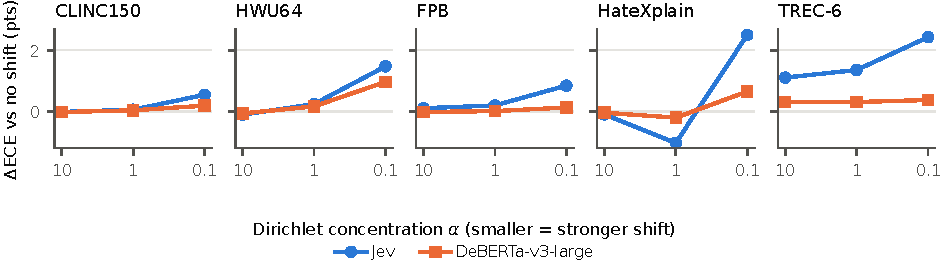
\includegraphics[width=\linewidth]{figures/fig3_shift.pdf}
  \caption{\textbf{Under stronger shift, Jev's calibration error grows more than DeBERTa-v3-large's on all five
  datasets, but this is not a zero-shot versus trained contrast: the TF-IDF classifier degrades more than Jev on two of
  them, and Tev1-4B more than Jev on FPB and TREC-6 (descriptive).}
  Change in ECE relative to a resampled no-shift control, mean over 200 Dirichlet draws per $\alpha$, raw probabilities.
  Only $\alpha=1$ is tested (\hyperref[tab:pa]{Table~\ref*{tab:pa}}); all systems in \hyperref[tab:exp2delta]{Table~\ref*{tab:exp2delta}}.}
  \label{fig:shift}
\end{figure}

\subsection{RQ3: Implicit-prior correction}
\label{sec:rq3}

\paragraph{EM with Jev's implicit prior lowers its calibration error under shift on the two datasets where that error is
highest.}
EM prior correction with Jev's implicit prior lowers Jev's ECE under shift on FPB by 2.7~points ($[-3.7,-1.6]$;
$p<0.007$; PA3) and on HateXplain by 1.8~points ($[-2.7,-0.8]$; $p<0.007$), the two datasets where Jev's unshifted ECE is
highest (0.095 and 0.279). On CLINC150 and HWU64, where its ECE is at most 0.036, the intervals lie between $-0.33$ and
$+0.54$ points; on TREC-6 the estimate is $-1.1$ points ($[-2.0,-0.3]$) but not significant after correction ($p=0.136$). Unlike PA1
and PA2, these effects keep their sign across shift scenarios: across the five other prior sets, the reduction is 1.7 to 2.5~points on FPB, 1.8 to 2.5 on HateXplain and 0.9 to 1.1 on TREC-6, with every unadjusted interval excluding zero
(\hyperref[tab:pasens]{Table~\ref*{tab:pasens}}). The FPB and HateXplain effects also exceed Jev's run-to-run variation in ECE (at most 0.6 and
1.1~points on these two datasets; \hyperref[tab:jevrepeat]{Table~\ref*{tab:jevrepeat}}). Descriptively, they appear to correct the shift rather
than Jev's label bias: on the resampled no-shift control, EM changes Jev's ECE by only $+0.1$ points on FPB and $+0.4$ on
HateXplain (descriptive; \hyperref[tab:emnoshift]{Table~\ref*{tab:emnoshift}}). The
correction is modest relative to the error it addresses: on HateXplain, Jev's mean ECE under shift falls from 0.271 to
0.254, whereas bias-corrected temperature scaling followed by EM, which needs development labels, reaches 0.071.
Descriptively, the same label-free correction lowers the shifted ECE of every zero-shot system on FPB and HateXplain, by
0.9 to 4.6~points (\hyperref[tab:exp2arms]{Table~\ref*{tab:exp2arms}}).

\paragraph{Most of the calibration gain under shift comes from calibrating on the development set (descriptive).}
The arms fall into two categories that should not be compared as alternatives: EM with the implicit prior is
\emph{label-free} and is the only option when no labelled data are available, whereas temperature scaling and BCTS+EM
are \emph{labelled} recalibration fitted on the labelled development set (the oracle uses the true target prior and is
only a reference). \hyperref[fig:arms]{Figure~\ref*{fig:arms}} and \hyperref[tab:exp2arms]{Table~\ref*{tab:exp2arms}} compare all five arms. On FPB and HateXplain, where most systems are
miscalibrated, bias-corrected temperature scaling followed by EM gives the lowest ECE under shift for 13 of the 14
system--dataset pairs, for example 0.035 for Nimble-9B on FPB against 0.271 without recalibration; the exception is
DeBERTa-v3-large on FPB, where temperature scaling alone is 0.2~points lower. Its gain is mostly the correction of
miscalibration that exists without shift: relative to its own no-shift control, the ECE of BCTS+EM still rises under shift,
by 1.5 to 3.1~points for the zero-shot systems on HateXplain, more than the raw probabilities do there, but it stays far
below the unrecalibrated level. Temperature scaling alone transfers less well: its ECE increases under shift more than
that of the raw probabilities for 31 of the 35 system--dataset pairs.

\begin{figure}[t]
  \centering
  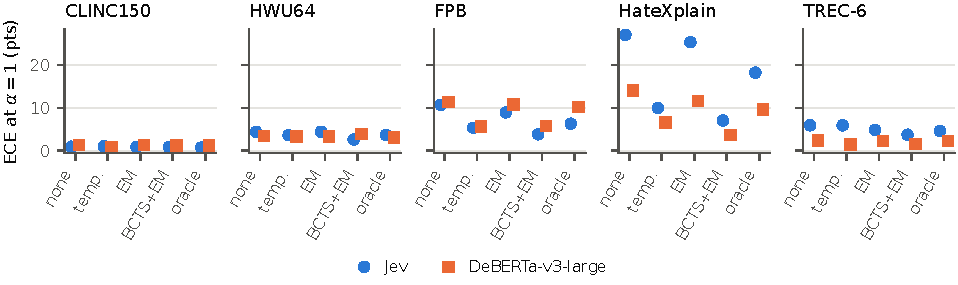
\includegraphics[width=\linewidth]{figures/fig4_arms.pdf}
  \caption{\textbf{Most of the calibration gain under shift comes from calibrating on the development set, not from
  correcting the prior (descriptive).} ECE under shift ($\alpha=1$, mean over 200 draws) for each recalibration arm.
  Label-free: EM, prior correction with the source prior (implicit for Jev, training prior for DeBERTa-v3-large).
  Labelled (fitted on the labelled development set): temp., temperature scaling; BCTS+EM, bias-corrected temperature
  scaling, then EM. Reference: oracle, true target prior (not deployable). All systems in \hyperref[tab:exp2arms]{Table~\ref*{tab:exp2arms}}.}
  \label{fig:arms}
\end{figure}

\section{Discussion}
\label{sec:discussion}

\paragraph{Is a typed decision model enough?}
Without task labels, Jev had the highest Macro-F1 point estimate among the zero-shot systems of the main comparison on
all five datasets, and
under moderate prevalence shift its calibration error and threshold risk were not distinguishable from those of
DeBERTa-v3-large after correction on four of the five. When the full training set is available, the fine-tuned
DeBERTa-v3-large still has the higher Macro-F1 point estimate everywhere, by 0.26~points on CLINC150 up to 18.9~points on
HateXplain. Whether a typed decision model is enough therefore depends on the task, on whether labels exist and on how
many. With our fixed training schedule, a fine-tuned DeBERTa-v3-large overtakes Jev with a few hundred labels on the
three-class tasks, needs 2{,}500--5{,}000 on HWU64 and is not clearly ahead on CLINC150 even with the full training set
(\hyperref[sec:rq4]{Section~\ref*{sec:rq4}}). For decisions within an intent group, then, a TDM is hard to beat with an
encoder fine-tuned on the task, but a QLoRA adapter on an open backbone overtakes Jev with at most 2{,}500 labels on
every dataset we tested, on CLINC150 only marginally and not under in-budget selection. These are five tasks, one backbone and three seeds for QLoRA; they show that a few thousand
labels can be enough, not how many a new task needs.

\paragraph{Why does the crossover rise with the number of classes?}
Two factors that our design cannot separate both point the same way. First, a fixed budget gives fewer examples per
class when there are more classes: 2{,}500 labels are on average 17 examples per class on CLINC150 but 833 on the
three-class tasks. Second, Jev leaves less room on the intent tasks, where its Macro-F1 is 0.978 and 0.908, than on
HateXplain (0.514), where it is weakest and the crossover comes earliest. The number of classes is also confounded with
domain and text length across our five datasets. The QLoRA result fits both factors: it starts from a model that
already reads the options zero-shot, so it does not have to learn each class from its few examples, and it overtakes
Jev earliest on the two datasets where Jev is least accurate. We offer this as a description of our five datasets, not
as a tested claim.

\paragraph{Why can decision training hurt?}
On FPB the two decision-trained models differ from their backbones in opposite directions: Tev1-4B's Macro-F1 is 10.0~points above Qwen3.5-4B's and Nimble-9B's is 12.0~points below Qwen3.5-9B's. The Tev1-4B gain, however, comes mostly from the base model's weak
score in the Tev1 format and disappears in generic formats (exploratory), so only the Nimble-9B result isolates an
effect of decision training. The Nimble release we test was trained on
2{,}676 synthetic examples, and FPB is labelled from an investor's point of view; one possible explanation is that the
synthetic data encode a different notion of positive and neutral financial news. The confusion matrices fit this
reading: the adapter mainly moves neutral sentences to the positive class (\hyperref[tab:fpbconf]{Table~\ref*{tab:fpbconf}}). We cannot test the
explanation itself without the vendors' training data. Both members of the pair run in the same 8-bit precision, so the comparison is matched, and
in bf16 the difference is nearly the same ($-11.7$~points; exploratory). What the paired design does establish is that,
for the same backbone, prompt and readout, decision training is not uniformly beneficial; a decision-trained variant
should be evaluated against its base model on the target task rather than assumed to be better, and the comparison
should also check that the base model is not handicapped by the TDM's prompt format.

\paragraph{Why does moderate shift matter so little?}
At $\alpha=1$ the target priors are centred on the training prior, so on average the shift is moderate, and for most
systems the calibration error under shift is dominated by the miscalibration they already have without shift; single
shifts, however, can be large (\hyperref[tab:excess]{Table~\ref*{tab:excess}}). Stronger shift ($\alpha=0.1$)
increases Jev's ECE more than DeBERTa-v3-large's on every dataset, but descriptively, and this is not a contrast between
zero-shot and trained systems: the trained TF-IDF classifier degrades more than Jev on two datasets, DeBERTa-v3-large is
the most stable system on three of the five, and on FPB and TREC-6 Tev1-4B degrades most of all systems (by 4.8 and 4.4~points, against 0.8 and 2.4 for Jev; \hyperref[tab:exp2delta]{Table~\ref*{tab:exp2delta}}). Two methodological points matter for such comparisons. First, resampling alone inflates
top-label ECE: on resampled data with no shift, ECE is 0.05 to 1.4~points higher than on the original test set (1.1~points for Jev on FPB, whose shift effect at $\alpha=1$ is 0.2~points), so shift effects must be measured against a
resampled control. Second, with only a few shift scenarios the result depends on which target priors are drawn
(\hyperref[sec:rq2]{Section~\ref*{sec:rq2}}), so conclusions should be stated for the shift distribution, not for a single draw.

\paragraph{Why does EM help most where the implicit prior is furthest from the truth?}
On FPB and HateXplain, Jev's implicit prior is far from the true class distribution (total-variation distance 0.18 and
0.23; \hyperref[tab:implicitprior]{Table~\ref*{tab:implicitprior}}), yet these are the datasets where EM with that prior helps most. This is less
paradoxical than it seems. The distance measures the model's label bias, not the quality of $\hat\pi_s$ as a reference
for EM. EM in \hyperref[eq:em]{Eq.~\ref*{eq:em}} rescales the posteriors by $\hat q/\hat\pi_s$, so what it needs is the prior with which
the model's own posteriors are consistent, which for a biased model is its own mean prediction and not the true prior.
Without shift, the mean prediction on the test set is close to $\hat\pi_s$ and EM leaves the posteriors almost
unchanged (\hyperref[tab:emnoshift]{Table~\ref*{tab:emnoshift}}); under shift, the change in the mean prediction is attributed to the shift, which
is what EM corrects. With the true prior in place of $\hat\pi_s$, EM would instead also try to remove the label bias,
which it cannot do reliably because the bias is not a change in class frequencies. Our data bear this out: with the
true class prior in place of the implicit one, EM raises the shifted ECE of every zero-shot system on FPB and
HateXplain above the uncorrected value (Jev on FPB: 0.172 against 0.107 without and 0.089 with the implicit prior;
exploratory, \hyperref[tab:emtrueprior]{Table~\ref*{tab:emtrueprior}}). EM then has the most to correct
where the shift moves the most probability mass between classes on which the model is calibrated differently. This is
the case for the three-class FPB and HateXplain, where Dirichlet draws at $\alpha=1$ often put most of the mass on one
class, and less so for the intent datasets, whose many classes and small ECE leave little to correct. We offer this as
an explanation consistent with our results, not as a tested claim.

\paragraph{What should a practitioner do?}
Four steps follow from our results. First, recalibrate on labelled data: bias-corrected temperature scaling followed by
EM, fitted on the labelled development sets, gave the lowest calibration error under shift for nearly every
system--dataset pair where calibration was poor. Second, without labels, EM with the model's implicit prior is a cheap
correction that lowered the shifted calibration error of every zero-shot system on FPB and HateXplain (descriptive;
tested only for Jev);
on the other datasets the intervals exclude harms larger than about half a point for Jev. Third, re-validate confidence
thresholds on target traffic: averaged over shifts, a single system's excess risk at 80\% coverage was at most 2.3~points at $\alpha=1$ (Nimble-9B on FPB), but individual shifts raised it by up to 35~points (Qwen3.5-4B on FPB) and by
up to 22~points for Jev on HateXplain (\hyperref[tab:excess]{Table~\ref*{tab:excess}}). Fourth, if labels can be
collected, test a task-tuned model against the TDM before choosing: in our five tasks, with 500 labels, a QLoRA adapter on
Qwen3.5-4B was above Jev on FPB and HateXplain, at most 0.8~points below it on the other three datasets (1.1 under
in-budget selection), and above both its frozen base and Tev1-4B on all five (on CLINC150 not resolved against Tev1-4B
under in-budget selection; \hyperref[fig:qlorabase]{Figure~\ref*{fig:qlorabase}}). How many labels a new task
needs is not something these five tasks can tell. On many-intent tasks, both comparisons assume that the right group
of intents is known. With a learned TF-IDF router, which misses the gold label's group on 6.2\% (CLINC150) and 7.0\%
(HWU64) of test examples, every system loses 5 to 6 accuracy points; on the missed examples, where the gold label is
not offered, the generative systems remain 70--84\% confident against 42--51\% for DeBERTa-v3-large (exploratory;
\hyperref[fig:router]{Figure~\ref*{fig:router}} in \hyperref[app:revision]{Appendix~\ref*{app:revision}}). A deployment
should therefore calibrate the routing step as well.

\paragraph{Relation to prior reports.}
Our FPB accuracy for Jev is consistent with \citet{deusser2026jev}, and so is our calibration pattern: like them, we
find Jev well calibrated where it is accurate (intent tasks) and miscalibrated where its accuracy is low (HateXplain). That decision training helps on some tasks and not others is consistent
with \citet{li2026llmasjev} and with the audit's conclusion that the typed readout itself has not shown an independent
accuracy advantage \citep{tang2026audit}; our paired design adds that the effect can be negative. The strength of BCTS
followed by EM matches \citet{alexandari2020maximum}; we observe it here also for zero-shot systems with an implicit
prior, but only descriptively, because our confirmatory test concerns plain EM.

\section{Limitations}
\label{sec:limitations}

\paragraph{Scope of systems and data.}
We study three TDMs, two open backbones and two trained classifiers; frontier generative APIs are out of scope. All
five datasets are English, public and human-labelled, and the TREC-6 and FPB test sets are small (500 and 970
examples), which widens their intervals. Public benchmarks may appear in the pretraining or decision-training data of
the models, which we can check only partly (\hyperref[app:runs]{Appendix~\ref*{app:runs}}); contamination would favour the zero-shot systems.

\paragraph{Task format.}
All results concern candidate-set decisions. On CLINC150 and HWU64 each example offers the 18--22 labels of a fixed label
group, not all 150 or 64 intents; the groups were chosen to prevent leakage of the gold label through the option list.
Full-label classification is harder for zero-shot systems, and other groupings could change the absolute numbers; we did
not test alternative groupings.

\paragraph{Shift model.}
We simulate prevalence shift by resampling test sets, so the label-shift assumption holds by construction. Real
deployments also change $p(x\mid y)$ (covariate or concept shift), under which prior correction can fail; our results
are therefore an optimistic case for prior correction. The confirmatory tests use one shift level ($\alpha=1$); the
stronger level is reported descriptively. A naturally or temporally shifted dataset, and alternative candidate
groupings, would test how far our conclusions transfer; both require new inference runs and are left to future work.

\paragraph{Design of the shift tests.}
The confirmatory PA1--PA3 estimand is conditional on one fixed set of 50 target priors, and its intervals reflect only
the finiteness of the test set. In hindsight this was a weakness of our design. Single priors move the Jev--DeBERTa
difference by several points on FPB and HateXplain (standard deviation 5.4 and 7.4~points across priors), so the frozen
set of 50 does not pin down the mean over the shift distribution: on FPB the confirmatory PA1 estimate is 1.7~points,
the average over 2{,}000 priors 0.4 (\hyperref[tab:papop]{Table~\ref*{tab:papop}}). The significant FPB results for PA1 and PA2 may therefore
reflect the particular prior set as much as a property of Jev. PA3 is less affected: across prior sets its estimate keeps
its sign and stays between 1.7 and 2.7~points on FPB. Future studies with a fixed protocol should target the mean over the shift
distribution, with the priors resampled inside the bootstrap or with many more priors, rather than a single prior set.

\paragraph{Models.}
Jev's version cannot be pinned (every call returned \texttt{jev-1.13.0}), and Jev is not deterministic: its probability
vectors differ between repeated calls on up to 81\% of examples, although its predictions rarely do. We run the two 9B
models in 8-bit precision to fit a 12\,GB GPU, whereas Nimble is distributed for bf16 inference; both members of the pair
share the precision, so the comparison is matched, but the size of the adapter effect in bf16 is untested and the
probabilities of 8-bit models can depend on the computation path. The vendors' training
data are not public, so we can show where decision training helps or hurts (for Nimble-9B on FPB, on the neutral class)
but not why.

\paragraph{Statistics.}
Bootstrap intervals hold quantities fitted on the development set fixed, and so understate total uncertainty; they are
not adjusted for multiplicity, whereas the reported significance is. Absence of a significant difference is not
evidence of equivalence beyond the width of the reported intervals.

\section{Conclusion}
\label{sec:conclusion}

We compared typed decision models with their own backbones and with trained classifiers on identical items and
candidate sets, under controlled prevalence shift and with 35 tests fixed before any test was computed. Vendor decision
training changed the same backbone in a task-dependent direction: with only an adapter between them, Nimble-9B was better
calibrated than Qwen3.5-9B on intent tasks and 12 Macro-F1~points worse on financial sentiment (RQ1). Under moderate
prevalence shift, Jev's calibration error and threshold risk grew significantly more than those of a fine-tuned DeBERTa
only on financial sentiment (by 1.7 and 2.5~points); this difference depended on the shift scenarios, and averaged over
many scenarios it was at most one point on every dataset (RQ2). A label-free EM correction with the model's implicit
prior lowered Jev's calibration error under shift by 2.7 and 1.8~points on the two datasets where it was highest,
consistently in sign across scenarios, but recalibration on labelled development data reduced it much further (RQ3).
The three typed decision models we tested are neither uniformly better than their backbones nor uniquely fragile under
prevalence shift; for calibration, their main weakness is the miscalibration they already have without shift. Whether
one is enough for a task is best decided by testing it against its base model and recalibrating it on labelled data
from the deployment setting.

\section*{Broader impact statement}
Typed decision models are built to make automated decisions inside software, for example routing, moderation and
triage. Our results show that their calibration and the error rate of confidence thresholds can change when the
deployment class distribution differs from the evaluation data, and that decision training can make a model worse on a
task. Deploying such models in consequential settings (moderation, finance, health) without validation on target data
can therefore cause harm; we recommend task-specific evaluation against a base model, recalibration on labelled data,
and monitoring of threshold error rates. HateXplain contains offensive text; we used it only for evaluation.

\section*{Reproducibility statement}
All datasets are public. Raw files, processed splits, label texts and candidate sets are pinned by SHA-256 hashes; the
frozen protocol, configurations and code are recorded in hash files, and every result was verified against them. Model
revisions are listed in \hyperref[tab:systems]{Table~\ref*{tab:systems}}; seeds are fixed throughout. We release the code, the protocol and
deviation log, and every per-example probability vector \todo{repository link}. Jev is a hosted model whose version
cannot be pinned and whose outputs are not deterministic (\hyperref[app:results]{Appendix~\ref*{app:results}}).


\bibliography{refs}
\bibliographystyle{tmlr}

\appendix
\section{Deviations from the frozen protocol}
\label{app:deviations}

The protocol (hypotheses, the 35-test family, configurations, data manifests and code) was frozen on 2026-10-08 at
07:45 UTC and recorded as SHA-256 hashes. While the local decoder runs were in progress, three code audits
were carried out; their findings led to one amendment, frozen at 10:58 UTC the same day. By then, test predictions of
Qwen3.5-4B and Tev1-4B had been produced, and the run log had printed their test accuracies. No test of the
35-test family, no shift analysis and no DeBERTa or Jev run had been carried out. The amendment did not change the code
used by the local decoder models, so all decoder runs, before and after it, use identical code; the DeBERTa and Jev
runs and every analysis use the amended version.
\paragraph{Chronology (UTC, from the run records).}
\begin{itemize}
  \item 2026-10-06: label texts frozen. 2026-10-07: data re-processed after a cleaning fix; candidate sets rebuilt as
  fixed groups after the leakage audit; pipeline checks, some on test splits (see the disclosure below).
  \item 2026-10-08 07:45: protocol v1.1 frozen (hash file).
  \item 2026-10-08 09:14--10:45: all Qwen3.5-4B and Tev1-4B predictions (development and test); 10:45: first
  Qwen3.5-9B run started.
  \item 2026-10-08 10:58: amendment v1.1.1 frozen; no test of the 35-test family and no shift analysis had been run.
  \item 2026-10-08 10:45--16:56: remaining local decoder predictions; latency timing completed on 2026-10-09.
  2026-10-09 to 10-10: DeBERTa-v3-large. 2026-10-13 05:23: TF-IDF.
  \item 2026-10-13 05:42: no-shift tables and P1/P2 for all systems except Jev; 05:47--07:50: all Jev runs;
  07:50--08:19: Jev's no-shift table and the descriptive shift experiment; 2026-10-13/14: PA1--PA3; 2026-10-14: Holm
  over all 35 tests.
  \item 2026-10-14, after all confirmatory results: prior-set sensitivity of PA1--PA3, HWU64 without the MASSIVE
  overlap, descriptive change in ECE and recalibration arms for all systems.
  \item 2026-10-15: distance of the implicit priors from the true class distribution, ECE range of the repeated Jev
  runs, excess-risk, Brier and NLL tables, TF-IDF grid extension to $10^5$ and $10^6$, average of PA1--PA3 over 2{,}000 priors, EM without
  shift, FPB confusion matrices, rank correlations between metrics. All are listed below and none changes a
  confirmatory result.
\end{itemize}

\paragraph{Amendment v1.1.1.}
\begin{itemize}
  \item \textbf{No-shift control.} The shift effect on ECE (the descriptive shift experiment and PA1) is measured against a no-shift control
  drawn with the same with-replacement resampler at the empirical class prior. The original protocol compared against
  the unresampled test set, which would have attributed resampling bias in top-label ECE to the shift.
  \item \textbf{Bootstrap size for PA1--PA3.} $B$ was raised from 1{,}000 to 10{,}000. With $B=1{,}000$ the smallest
  non-zero two-sided $p$ ($2/B=0.002$) is above Holm's first threshold ($0.05/35\approx0.0014$).
  \item \textbf{Failed-run rule for DeBERTa.} The majority-class threshold is computed within each example's candidate
  set, on the same scale as the model's accuracy (previously the two were on different scales for CLINC150 and HWU64).
  No full-data run failed under either rule.
  \item \textbf{Jev transport errors.} Network errors are never classified as refusals. No Jev request failed or was
  refused in the final runs.
  \item \textbf{No-shift metrics.} The specified treatment of refused requests (counted as wrong and abstained) was
  implemented; no request was refused. The confirmatory scope of H3 was narrowed in wording to plain EM on Jev, and
  the AURC definition was stated exactly.
\end{itemize}
\textbf{Analyses added after the results were known.} The following analyses were added after the confirmatory results
had been computed, in response to reviews of the draft; all are labelled exploratory or descriptive and none
changes a confirmatory result: the prior-set sensitivity of PA1--PA3 (\hyperref[tab:pasens]{Table~\ref*{tab:pasens}}) and their average over
2{,}000 target priors (\hyperref[tab:papop]{Table~\ref*{tab:papop}}); the HWU64 analysis without the MASSIVE overlap (required by the protocol
but run only at this stage; \hyperref[tab:hwu64]{Table~\ref*{tab:hwu64}}); the descriptive shift-experiment summaries for all systems
(\hyperref[tab:exp2delta]{Tables~\ref*{tab:exp2delta}}--\nobreak\ref{tab:nll}); the distance of each implicit prior from the true class distribution
(\hyperref[tab:implicitprior]{Table~\ref*{tab:implicitprior}}); the effect of EM without shift (\hyperref[tab:emnoshift]{Table~\ref*{tab:emnoshift}}); the FPB confusion matrices
of the Nimble pair (\hyperref[tab:fpbconf]{Table~\ref*{tab:fpbconf}}); the ECE range of the repeated Jev runs
(\hyperref[tab:jevrepeat]{Table~\ref*{tab:jevrepeat}}); the rank correlations between metrics
(\hyperref[tab:exp1full]{Table~\ref*{tab:exp1full}}); a check that the PA estimates are not an artefact of
resampling twice (PA1--PA3 recomputed without the bootstrap base on FPB, HateXplain and TREC-6; the estimates agree);
and the extension of the TF-IDF regularisation grid to $10^5$ and $10^6$
(\hyperref[sec:protocol]{Section~\ref*{sec:protocol}}).

\textbf{Disclosure.} During pipeline development, before the freeze, checks of the code were run on \emph{test}
splits: Jev on the full FPB test split and on 5 to 10 test examples of CLINC150, FPB and HateXplain; Qwen3.5-4B and
Tev1-4B on 5 FPB test examples each; a DeBERTa-v3-large model trained on 100 examples, on the FPB test split; TF-IDF
on all five test splits in three pipeline runs, whose test scores were printed; and early versions of PA1--PA3 and
the descriptive shift experiment on FPB. Two design changes followed these checks: fixed target priors for PA1--PA3,
because of the width of the intervals under the earlier design, and the extension of the TF-IDF grid from $10^3$ to
$10^4$, because the value selected on the development set lay at the edge of the grid. Neither change was based on
the direction or size of a test estimate. From then on, pipeline checks used only the development split, and all reported test results come from the
frozen protocol.

\FloatBarrier
\section{Additional results}
\label{app:results}

\begin{table}[htbp]
  \centering
  \caption{\textbf{Fourteen of the 35 confirmatory tests are significant after Holm correction.} Paired differences in percentage points (TDM $-$ base for P1/P2; Jev $-$
  DeBERTa-v3-large for PA1/PA2; EM $-$ none for PA3) with unadjusted 95\% bootstrap intervals, raw two-sided $p$ and
  Holm-adjusted $p$ over the 35 tests.}
  \label{tab:alltests}
  \scriptsize
  \begin{tabular}{llrcrr}
\toprule
Test & Dataset & $\Delta$ (points) & 95\% CI & $p$ & Holm $p$ \\
\midrule
\rowcolor{rowhl} P1-F1 & CLINC150 & +2.48 & [+1.94, +3.10] & $<$0.0002 & $<$0.007 \\
\rowcolor{rowhl} P1-F1 & HWU64 & +2.84 & [+1.10, +4.78] & 0.002 & 0.040 \\
\rowcolor{rowhl} P1-F1 & FPB & +9.99 & [+7.35, +12.69] & $<$0.0002 & $<$0.007 \\
P1-F1 & HateXplain & +1.69 & [$-$0.16, +3.52] & 0.077 & 1.000 \\
P1-F1 & TREC-6 & +0.65 & [$-$2.92, +4.44] & 0.724 & 1.000 \\
\midrule
P1-ECE & CLINC150 & $-$0.34 & [$-$0.84, +0.21] & 0.255 & 1.000 \\
P1-ECE & HWU64 & $-$1.87 & [$-$3.29, $-$0.19] & 0.028 & 0.479 \\
\rowcolor{rowhl} P1-ECE & FPB & $-$13.19 & [$-$15.75, $-$10.39] & $<$0.0002 & $<$0.007 \\
\rowcolor{rowhl} P1-ECE & HateXplain & $-$3.23 & [$-$5.19, $-$1.37] & 0.001 & 0.029 \\
P1-ECE & TREC-6 & +0.12 & [$-$2.97, +2.37] & 0.796 & 1.000 \\
\midrule
\rowcolor{rowhl} P2-F1 & CLINC150 & +0.69 & [+0.23, +1.17] & 0.001 & 0.029 \\
P2-F1 & HWU64 & +1.14 & [$-$0.64, +3.03] & 0.195 & 1.000 \\
\rowcolor{rowhl} P2-F1 & FPB & $-$11.97 & [$-$14.61, $-$9.28] & $<$0.0002 & $<$0.007 \\
P2-F1 & HateXplain & $-$1.66 & [$-$3.23, $-$0.07] & 0.039 & 0.630 \\
P2-F1 & TREC-6 & $-$3.11 & [$-$6.99, +0.69] & 0.100 & 1.000 \\
\midrule
\rowcolor{rowhl} P2-ECE & CLINC150 & $-$1.22 & [$-$1.52, $-$0.63] & $<$0.0002 & $<$0.007 \\
\rowcolor{rowhl} P2-ECE & HWU64 & $-$4.22 & [$-$5.59, $-$2.50] & $<$0.0002 & $<$0.007 \\
\rowcolor{rowhl} P2-ECE & FPB & +9.56 & [+6.77, +12.05] & $<$0.0002 & $<$0.007 \\
P2-ECE & HateXplain & $-$0.36 & [$-$1.94, +1.21] & 0.636 & 1.000 \\
P2-ECE & TREC-6 & $-$1.84 & [$-$3.67, +1.63] & 0.440 & 1.000 \\
\midrule
PA1 & CLINC150 & +0.09 & [$-$0.02, +0.20] & 0.104 & 1.000 \\
PA1 & HWU64 & +0.11 & [$-$0.30, +0.50] & 0.592 & 1.000 \\
\rowcolor{rowhl} PA1 & FPB & +1.71 & [+0.98, +2.49] & $<$0.0002 & $<$0.007 \\
PA1 & HateXplain & $-$0.78 & [$-$1.29, $-$0.26] & 0.004 & 0.080 \\
PA1 & TREC-6 & +1.01 & [+0.26, +1.85] & 0.007 & 0.136 \\
\midrule
PA2 & CLINC150 & 0.00 & [$-$0.04, +0.04] & 0.938 & 1.000 \\
PA2 & HWU64 & +0.01 & [$-$0.21, +0.23] & 0.969 & 1.000 \\
\rowcolor{rowhl} PA2 & FPB & +2.49 & [+1.83, +3.16] & $<$0.0002 & $<$0.007 \\
PA2 & HateXplain & $-$0.55 & [$-$0.98, $-$0.14] & 0.010 & 0.187 \\
PA2 & TREC-6 & +0.55 & [$-$0.06, +1.30] & 0.086 & 1.000 \\
\midrule
PA3 & CLINC150 & $-$0.12 & [$-$0.29, +0.03] & 0.122 & 1.000 \\
PA3 & HWU64 & +0.12 & [$-$0.33, +0.54] & 0.546 & 1.000 \\
\rowcolor{rowhl} PA3 & FPB & $-$2.65 & [$-$3.74, $-$1.61] & $<$0.0002 & $<$0.007 \\
\rowcolor{rowhl} PA3 & HateXplain & $-$1.75 & [$-$2.71, $-$0.82] & $<$0.0002 & $<$0.007 \\
PA3 & TREC-6 & $-$1.06 & [$-$1.96, $-$0.28] & 0.007 & 0.136 \\
\bottomrule
\end{tabular}

\end{table}

\begin{table}[htbp]
  \centering
  \caption{\textbf{Accuracy and MCC rank the seven analysed systems almost as Macro-F1 does (Spearman $\rho\ge0.75$ on
  every dataset; descriptive), whereas NLL, which penalises confident errors, ranks them differently on HWU64 and
  HateXplain ($\rho=0.29$ and $0.32$).} Test-set metrics for all systems, no shift. $^\ast$Exploratory: a later Nimble
  release whose training data include public TREC questions, which may explain its TREC-6 score; it is not part of any
  confirmatory test or of the rank correlations. Acc@80: accuracy on the 80\% most confident examples.}
  \label{tab:exp1full}
  \scriptsize
  \setlength{\tabcolsep}{3pt}
  \begin{tabular}{llrrrrrrrr}
\toprule
Dataset & System & Acc$\uparrow$ & F1$\uparrow$ & MCC$\uparrow$ & ECE$\downarrow$ & Brier$\downarrow$ & NLL$\downarrow$ & AURC$\downarrow$ & Acc@80$\uparrow$ \\
\midrule
CLINC150 & Jev & 0.978 & 0.978 & 0.978 & 0.007 & 0.032 & 0.152 & 0.004 & 0.997 \\
 & Tev1-4B & 0.964 & 0.964 & 0.963 & 0.008 & 0.055 & 0.130 & 0.003 & 0.997 \\
 & Nimble-9B & 0.962 & 0.962 & 0.961 & 0.008 & 0.060 & 0.140 & 0.004 & 0.996 \\
 & Nimble-9B (main)$^\ast$ & 0.969 & 0.969 & 0.968 & 0.010 & 0.050 & 0.123 & 0.002 & 0.997 \\
 & Qwen3.5-4B & 0.939 & 0.939 & 0.939 & 0.011 & 0.089 & 0.233 & 0.007 & 0.994 \\
 & Qwen3.5-9B & 0.955 & 0.955 & 0.955 & 0.020 & 0.067 & 0.176 & 0.005 & 0.995 \\
 & DeBERTa-v3-large & 0.980 & 0.980 & 0.980 & 0.013 & 0.031 & 0.105 & 0.002 & 0.997 \\
 & TF-IDF + LR & 0.950 & 0.950 & 0.949 & 0.015 & 0.077 & 0.189 & 0.005 & 0.993 \\
\midrule
HWU64 & Jev & 0.911 & 0.908 & 0.910 & 0.036 & 0.138 & 0.640 & 0.024 & 0.976 \\
 & Tev1-4B & 0.891 & 0.895 & 0.890 & 0.040 & 0.168 & 0.423 & 0.021 & 0.962 \\
 & Nimble-9B & 0.897 & 0.896 & 0.896 & 0.035 & 0.165 & 0.436 & 0.026 & 0.956 \\
 & Nimble-9B (main)$^\ast$ & 0.896 & 0.896 & 0.895 & 0.042 & 0.156 & 0.360 & 0.017 & 0.974 \\
 & Qwen3.5-4B & 0.862 & 0.866 & 0.860 & 0.058 & 0.216 & 0.596 & 0.029 & 0.944 \\
 & Qwen3.5-9B & 0.880 & 0.884 & 0.879 & 0.078 & 0.200 & 0.616 & 0.028 & 0.956 \\
 & DeBERTa-v3-large & 0.943 & 0.939 & 0.942 & 0.030 & 0.094 & 0.269 & 0.009 & 0.984 \\
 & TF-IDF + LR & 0.901 & 0.900 & 0.900 & 0.098 & 0.177 & 0.444 & 0.019 & 0.966 \\
\midrule
FPB & Jev & 0.744 & 0.752 & 0.608 & 0.095 & 0.373 & 0.745 & 0.120 & 0.795 \\
 & Tev1-4B & 0.715 & 0.735 & 0.597 & 0.072 & 0.378 & 0.582 & 0.141 & 0.751 \\
 & Nimble-9B & 0.608 & 0.629 & 0.508 & 0.263 & 0.612 & 1.138 & 0.205 & 0.644 \\
 & Nimble-9B (main)$^\ast$ & 0.652 & 0.683 & 0.542 & 0.167 & 0.509 & 0.849 & 0.194 & 0.688 \\
 & Qwen3.5-4B & 0.597 & 0.635 & 0.499 & 0.204 & 0.585 & 1.107 & 0.252 & 0.640 \\
 & Qwen3.5-9B & 0.743 & 0.749 & 0.607 & 0.168 & 0.403 & 0.821 & 0.115 & 0.818 \\
 & DeBERTa-v3-large & 0.875 & 0.870 & 0.776 & 0.111 & 0.234 & 0.634 & 0.045 & 0.920 \\
 & TF-IDF + LR & 0.753 & 0.693 & 0.538 & 0.167 & 0.401 & 0.990 & 0.123 & 0.817 \\
\midrule
HateXplain & Jev & 0.535 & 0.514 & 0.348 & 0.279 & 0.704 & 2.992 & 0.330 & 0.574 \\
 & Tev1-4B & 0.464 & 0.458 & 0.235 & 0.214 & 0.702 & 1.297 & 0.435 & 0.501 \\
 & Nimble-9B & 0.490 & 0.470 & 0.284 & 0.336 & 0.800 & 1.735 & 0.416 & 0.521 \\
 & Nimble-9B (main)$^\ast$ & 0.504 & 0.495 & 0.286 & 0.266 & 0.721 & 1.428 & 0.397 & 0.532 \\
 & Qwen3.5-4B & 0.460 & 0.441 & 0.237 & 0.247 & 0.740 & 1.415 & 0.457 & 0.493 \\
 & Qwen3.5-9B & 0.501 & 0.487 & 0.289 & 0.340 & 0.803 & 1.764 & 0.409 & 0.522 \\
 & DeBERTa-v3-large & 0.710 & 0.703 & 0.563 & 0.141 & 0.433 & 0.769 & 0.161 & 0.774 \\
 & TF-IDF + LR & 0.663 & 0.645 & 0.486 & 0.069 & 0.461 & 0.814 & 0.200 & 0.720 \\
\midrule
TREC-6 & Jev & 0.930 & 0.922 & 0.912 & 0.042 & 0.116 & 0.342 & 0.016 & 0.970 \\
 & Tev1-4B & 0.884 & 0.889 & 0.858 & 0.038 & 0.190 & 0.361 & 0.042 & 0.927 \\
 & Nimble-9B & 0.848 & 0.872 & 0.814 & 0.043 & 0.207 & 0.370 & 0.037 & 0.925 \\
 & Nimble-9B (main)$^\ast$ & 0.968 & 0.963 & 0.960 & 0.017 & 0.056 & 0.129 & 0.006 & 0.990 \\
 & Qwen3.5-4B & 0.880 & 0.882 & 0.853 & 0.037 & 0.177 & 0.363 & 0.029 & 0.950 \\
 & Qwen3.5-9B & 0.888 & 0.903 & 0.862 & 0.061 & 0.174 & 0.355 & 0.026 & 0.960 \\
 & DeBERTa-v3-large & 0.976 & 0.971 & 0.970 & 0.021 & 0.041 & 0.153 & 0.010 & 0.990 \\
 & TF-IDF + LR & 0.894 & 0.891 & 0.868 & 0.071 & 0.176 & 0.449 & 0.022 & 0.973 \\
\bottomrule
\end{tabular}

\end{table}

\begin{table}[htbp]
  \centering
  \caption{\textbf{DeBERTa-v3-large is stable across seeds.} Test Macro-F1 of the five full-data seeds; all analyses use
  seed 1001.}
  \label{tab:seeds}
  \scriptsize
  \begin{tabular}{lrrrrrr}
\toprule
Dataset & seed 1001 & 1002 & 1003 & 1004 & 1005 & mean $\pm$ SD \\
\midrule
CLINC150 & 0.980 & 0.981 & 0.983 & 0.982 & 0.981 & 0.981 $\pm$ 0.001 \\
HWU64 & 0.939 & 0.943 & 0.954 & 0.943 & 0.942 & 0.944 $\pm$ 0.006 \\
FPB & 0.870 & 0.854 & 0.857 & 0.865 & 0.868 & 0.863 $\pm$ 0.007 \\
HateXplain & 0.703 & 0.700 & 0.700 & 0.711 & 0.700 & 0.703 $\pm$ 0.005 \\
TREC-6 & 0.971 & 0.978 & 0.974 & 0.971 & 0.959 & 0.971 $\pm$ 0.007 \\
\bottomrule
\end{tabular}

\end{table}

\begin{table}[htbp]
  \centering
  \caption{\textbf{Jev's predictions are nearly stable across repeated calls, its probabilities are not, and its ECE
  varies by up to 1.2~points between runs.} Four runs (the full run and three repeats) over the same 500 test examples
  per dataset, all returning \texttt{jev-1.13.0}; accuracy shown for the three repeats, ECE range over all four runs.}
  \label{tab:jevrepeat}
  \scriptsize
  \begin{tabular}{lrrrrlc}
\toprule
Dataset & $n$ & same prediction & same prob.\ vector & max $|\Delta p|$ & accuracy (3 repeats) & ECE range (4 runs) \\
\midrule
CLINC150 & 500 & 99.8\% & 87.4\% & 0.12 & 0.972 / 0.970 / 0.972 & 0.012--0.015 \\
HWU64 & 500 & 99.6\% & 72.2\% & 0.20 & 0.918 / 0.920 / 0.916 & 0.039--0.049 \\
FPB & 500 & 97.6\% & 27.4\% & 0.16 & 0.738 / 0.738 / 0.736 & 0.110--0.116 \\
HateXplain & 500 & 96.4\% & 19.4\% & 0.29 & 0.538 / 0.532 / 0.532 & 0.271--0.282 \\
TREC-6 & 500 & 98.2\% & 63.8\% & 0.15 & 0.926 / 0.928 / 0.926 & 0.030--0.042 \\
\bottomrule
\end{tabular}

\end{table}

\begin{table}[htbp]
  \centering
  \caption{\textbf{Under the strongest shift, the calibration error grows for every system on four of the five
  datasets (TF-IDF on FPB is unchanged), and DeBERTa-v3-large is the most stable on three of the five datasets
  (descriptive).} Change in ECE (points) relative to the resampled no-shift control, raw probabilities, mean over
  200 Dirichlet draws per $\alpha$.}
  \label{tab:exp2delta}
  \scriptsize
  \setlength{\tabcolsep}{3pt}
  \begin{tabular}{lrrrrrrrrrr}
\toprule
 & \multicolumn{2}{c}{CLINC150} & \multicolumn{2}{c}{HWU64} & \multicolumn{2}{c}{FPB} & \multicolumn{2}{c}{HateXplain} & \multicolumn{2}{c}{TREC-6} \\
\cmidrule(lr){2-3} \cmidrule(lr){4-5} \cmidrule(lr){6-7} \cmidrule(lr){8-9} \cmidrule(lr){10-11}
System & $\alpha$=1 & 0.1 & $\alpha$=1 & 0.1 & $\alpha$=1 & 0.1 & $\alpha$=1 & 0.1 & $\alpha$=1 & 0.1 \\
\midrule
Jev & +0.1 & +0.5 & +0.2 & +1.5 & +0.2 & +0.8 & $-$1.0 & +2.5 & +1.4 & +2.4 \\
Tev1-4B & +0.1 & +0.9 & +0.3 & +1.9 & +1.1 & +4.8 & $-$0.8 & +2.0 & +1.9 & +4.4 \\
Nimble-9B & +0.1 & +1.0 & +0.4 & +2.0 & +0.5 & +1.0 & $-$1.2 & +2.5 & +0.8 & +2.6 \\
Qwen3.5-4B & +0.3 & +1.3 & +0.3 & +1.7 & +0.8 & +3.9 & $-$0.9 & +3.7 & +0.8 & +2.7 \\
Qwen3.5-9B & +0.1 & +0.4 & +0.1 & +0.8 & +0.2 & +0.3 & $-$1.0 & +1.9 & +0.2 & +1.2 \\
DeBERTa-v3-large & 0.0 & +0.2 & +0.2 & +1.0 & 0.0 & +0.1 & $-$0.2 & +0.7 & +0.3 & +0.4 \\
TF-IDF + LR & +0.1 & +1.1 & +0.3 & +1.4 & $-$0.1 & 0.0 & +0.8 & +3.3 & +0.9 & +1.4 \\
\bottomrule
\end{tabular}

\end{table}

\begin{table}[htbp]
  \centering
  \caption{\textbf{Bias-corrected temperature scaling followed by EM gives the lowest calibration error under shift for
  most systems, and EM with the implicit prior helps every zero-shot system on FPB and HateXplain (descriptive).} ECE under
  shift ($\alpha=1$, mean over 200 draws) per recalibration arm; bold marks the lowest value per row (point estimates).}
  \label{tab:exp2arms}
  \scriptsize
  \begin{tabular}{llrrrrr}
\toprule
Dataset & System & none & temp. & EM & BCTS+EM & oracle \\
\midrule
CLINC150 & Jev & 0.009 & 0.010 & 0.008 & 0.008 & \textbf{0.007} \\
 & Tev1-4B & 0.011 & 0.010 & 0.011 & 0.010 & \textbf{0.010} \\
 & Nimble-9B & 0.011 & \textbf{0.009} & 0.012 & 0.017 & 0.010 \\
 & Qwen3.5-4B & 0.016 & 0.015 & 0.015 & 0.014 & \textbf{0.012} \\
 & Qwen3.5-9B & 0.022 & \textbf{0.011} & 0.020 & 0.014 & 0.017 \\
 & DeBERTa-v3-large & 0.014 & \textbf{0.008} & 0.013 & 0.012 & 0.012 \\
 & TF-IDF + LR & 0.019 & 0.018 & 0.015 & 0.018 & \textbf{0.014} \\
\midrule
HWU64 & Jev & 0.044 & 0.036 & 0.044 & \textbf{0.026} & 0.037 \\
 & Tev1-4B & 0.047 & 0.037 & 0.048 & \textbf{0.034} & 0.039 \\
 & Nimble-9B & 0.045 & 0.037 & 0.047 & \textbf{0.029} & 0.037 \\
 & Qwen3.5-4B & 0.064 & 0.040 & 0.063 & \textbf{0.036} & 0.047 \\
 & Qwen3.5-9B & 0.083 & 0.035 & 0.081 & \textbf{0.030} & 0.064 \\
 & DeBERTa-v3-large & 0.035 & 0.033 & 0.033 & 0.039 & \textbf{0.030} \\
 & TF-IDF + LR & 0.102 & 0.044 & 0.060 & \textbf{0.041} & 0.075 \\
\midrule
FPB & Jev & 0.107 & 0.054 & 0.089 & \textbf{0.038} & 0.063 \\
 & Tev1-4B & 0.090 & 0.090 & 0.081 & \textbf{0.033} & 0.045 \\
 & Nimble-9B & 0.271 & 0.132 & 0.243 & \textbf{0.035} & 0.101 \\
 & Qwen3.5-4B & 0.217 & 0.110 & 0.185 & \textbf{0.041} & 0.065 \\
 & Qwen3.5-9B & 0.173 & 0.067 & 0.153 & \textbf{0.041} & 0.115 \\
 & DeBERTa-v3-large & 0.114 & \textbf{0.056} & 0.108 & 0.058 & 0.103 \\
 & TF-IDF + LR & 0.168 & 0.075 & 0.151 & \textbf{0.047} & 0.138 \\
\midrule
HateXplain & Jev & 0.271 & 0.100 & 0.254 & \textbf{0.071} & 0.183 \\
 & Tev1-4B & 0.208 & 0.094 & 0.162 & \textbf{0.076} & 0.107 \\
 & Nimble-9B & 0.325 & 0.110 & 0.306 & \textbf{0.069} & 0.213 \\
 & Qwen3.5-4B & 0.239 & 0.101 & 0.203 & \textbf{0.064} & 0.127 \\
 & Qwen3.5-9B & 0.331 & 0.093 & 0.315 & \textbf{0.058} & 0.239 \\
 & DeBERTa-v3-large & 0.140 & 0.066 & 0.116 & \textbf{0.037} & 0.097 \\
 & TF-IDF + LR & 0.082 & 0.067 & 0.062 & \textbf{0.047} & 0.057 \\
\midrule
TREC-6 & Jev & 0.059 & 0.059 & 0.049 & \textbf{0.037} & 0.046 \\
 & Tev1-4B & 0.067 & 0.070 & 0.067 & \textbf{0.043} & 0.048 \\
 & Nimble-9B & 0.062 & 0.048 & 0.056 & 0.048 & \textbf{0.047} \\
 & Qwen3.5-4B & 0.059 & 0.050 & 0.053 & \textbf{0.049} & 0.052 \\
 & Qwen3.5-9B & 0.066 & 0.054 & 0.060 & \textbf{0.045} & 0.055 \\
 & DeBERTa-v3-large & 0.024 & \textbf{0.014} & 0.023 & 0.016 & 0.023 \\
 & TF-IDF + LR & 0.085 & 0.056 & 0.080 & \textbf{0.043} & 0.074 \\
\bottomrule
\end{tabular}

\end{table}

\begin{table}[htbp]
  \centering
  \caption{\textbf{The confirmatory PA estimates and the 200-draw descriptive experiment agree in direction on every
  dataset, but their size depends on the set of target priors.} PA rows: 50 fixed priors with the class-stratified
  bootstrap; descriptive rows: 200 independent Dirichlet draws on the full test set (points). Prior-set sensitivity:
  \hyperref[sec:rq2]{Section~\ref*{sec:rq2}}.}
  \label{tab:pavsexp2}
  \scriptsize
  \begin{tabular}{lccccc}
\toprule
Quantity (points) & CLINC150 & HWU64 & FPB & HateXplain & TREC-6 \\
\midrule
PA1 ($\Delta$ECE, Jev $-$ DeBERTa): 50 fixed priors & +0.1 & +0.1 & +1.7 & $-$0.8 & +1.0 \\
\quad 200 descriptive draws &0.0 & +0.1 & +0.2 & $-$0.8 & +1.0 \\
PA2 (excess risk, Jev $-$ DeBERTa): 50 fixed priors & 0.0 & 0.0 & +2.5 & $-$0.6 & +0.5 \\
\quad 200 descriptive draws &0.0 & 0.0 & +0.4 & $-$0.7 & +0.4 \\
PA3 (ECE, Jev EM $-$ none): 50 fixed priors & $-$0.1 & +0.1 & $-$2.7 & $-$1.8 & $-$1.1 \\
\quad 200 descriptive draws &$-$0.1 & 0.0 & $-$1.8 & $-$1.7 & $-$1.1 \\
\bottomrule
\end{tabular}

\end{table}

\begin{table}[htbp]
  \centering
  \caption{\textbf{Averaged over many target priors, the Jev--DeBERTa difference under moderate shift is small on every
  dataset, while the EM effect (PA3) stays clearly negative on FPB and HateXplain (exploratory).} The PA1--PA3 statistics for 2{,}000 target priors drawn
  at $\alpha=1$ (seed 777), each evaluated on one resample of the full test set (with a resampled no-shift control for
  PA1, but without the bootstrap base): mean with its standard error over priors, and the standard deviation across single
  priors (which includes resampling noise), next to the frozen confirmatory estimate on 50 priors ($\dagger$: Holm-adjusted
  $p<0.05$). Points.}
  \label{tab:papop}
  \scriptsize
  \begin{tabular}{llccccc}
\toprule
Test & Estimate & CLINC150 & HWU64 & FPB & HateXplain & TREC-6 \\
\midrule
PA1 & frozen 50 priors & +0.1 & +0.1 & \textbf{+1.7}$^\dagger$ & $-$0.8 & +1.0 \\
 & 2{,}000 priors: mean (SE) & 0.0 (0.0) & +0.1 (0.0) & +0.4 (0.1) & 0.0 (0.2) & +1.0 (0.0) \\
 & SD across priors & 0.4 & 1.4 & 5.4 & 7.4 & 1.7 \\
\midrule
PA2 & frozen 50 priors & 0.0 & 0.0 & \textbf{+2.5}$^\dagger$ & $-$0.6 & +0.5 \\
 & 2{,}000 priors: mean (SE) & 0.0 (0.0) & 0.0 (0.0) & +0.5 (0.2) & +0.4 (0.2) & +0.5 (0.0) \\
 & SD across priors & 0.2 & 0.9 & 7.6 & 9.8 & 1.3 \\
\midrule
PA3 & frozen 50 priors & $-$0.1 & +0.1 & \textbf{$-$2.7}$^\dagger$ & \textbf{$-$1.8}$^\dagger$ & $-$1.1 \\
 & 2{,}000 priors: mean (SE) & $-$0.1 (0.0) & 0.0 (0.0) & $-$1.7 (0.1) & $-$2.0 (0.1) & $-$1.0 (0.0) \\
 & SD across priors & 0.2 & 0.8 & 3.9 & 3.8 & 1.3 \\
\bottomrule
\end{tabular}

\end{table}

\begin{table}[htbp]
  \centering
  \caption{\textbf{Averaged over shifts, the excess risk of a fixed confidence threshold is small, but single shifts can
  raise it by up to 35~points (descriptive).} Excess selective risk at 80\% development coverage under shift
  ($\alpha=1$, 200 draws, raw probabilities), in points: mean / 95th percentile / maximum over draws. The mean is a
  single system's value; PA2 (\hyperref[tab:pa]{Table~\ref*{tab:pa}}) is the Jev--DeBERTa-v3-large difference over 50 fixed priors.}
  \label{tab:excess}
  \scriptsize
  \setlength{\tabcolsep}{3pt}
  \begin{tabular}{lccccc}
\toprule
System & CLINC150 & HWU64 & FPB & HateXplain & TREC-6 \\
\midrule
Jev & 0.0 / 0.3 / 0.6 & 0.0 / 1.3 / 2.3 & +0.4 / 9.6 / 12.4 & $-$0.9 / 19.5 / 21.8 & +0.7 / 2.8 / 4.1 \\
Tev1-4B & 0.0 / 0.3 / 0.6 & $-$0.1 / 1.7 / 2.9 & +1.0 / 17.1 / 21.3 & $-$0.6 / 12.1 / 16.1 & +0.9 / 5.3 / 7.9 \\
Nimble-9B & 0.0 / 0.2 / 0.7 & +0.1 / 2.4 / 5.6 & +2.3 / 28.4 / 33.0 & $-$1.1 / 17.4 / 20.2 & 0.0 / 2.9 / 4.9 \\
Qwen3.5-4B & 0.0 / 0.3 / 0.7 & 0.0 / 2.0 / 4.8 & +2.1 / 27.3 / 34.7 & $-$1.0 / 17.2 / 19.2 & +0.4 / 3.2 / 4.8 \\
Qwen3.5-9B & 0.0 / 0.3 / 0.5 & +0.1 / 2.3 / 4.4 & +0.5 / 9.3 / 11.2 & $-$1.0 / 15.7 / 17.6 & 0.0 / 2.6 / 3.7 \\
DeBERTa-v3-large & 0.0 / 0.2 / 0.4 & $-$0.1 / 0.9 / 2.1 & 0.0 / 3.4 / 5.9 & $-$0.2 / 10.2 / 12.6 & +0.3 / 2.1 / 3.8 \\
TF-IDF + LR & 0.0 / 0.5 / 0.7 & $-$0.1 / 1.4 / 2.3 & +0.1 / 12.5 / 17.7 & $-$0.1 / 15.0 / 21.1 & +0.8 / 4.9 / 9.4 \\
\bottomrule
\end{tabular}

\end{table}

\begin{table}[htbp]
  \centering
  \caption{\textbf{Brier score under shift follows the same pattern as ECE: small changes at $\alpha=1$, larger ones at
  $\alpha=0.1$, mostly for the zero-shot systems on HateXplain (descriptive).} Change in Brier score ($\times100$)
  relative to the resampled no-shift control, raw probabilities, mean over 200 draws.}
  \label{tab:brier}
  \scriptsize
  \setlength{\tabcolsep}{3pt}
  \begin{tabular}{lrrrrrrrrrr}
\toprule
 & \multicolumn{2}{c}{CLINC150} & \multicolumn{2}{c}{HWU64} & \multicolumn{2}{c}{FPB} & \multicolumn{2}{c}{HateXplain} & \multicolumn{2}{c}{TREC-6} \\
\cmidrule(lr){2-3} \cmidrule(lr){4-5} \cmidrule(lr){6-7} \cmidrule(lr){8-9} \cmidrule(lr){10-11}
System & $\alpha$=1 & 0.1 & $\alpha$=1 & 0.1 & $\alpha$=1 & 0.1 & $\alpha$=1 & 0.1 & $\alpha$=1 & 0.1 \\
\midrule
Jev & 0.0 & +0.1 & $-$0.2 & $-$0.6 & 0.0 & +0.3 & $-$2.0 & +3.7 & +1.7 & +1.9 \\
Tev1-4B & $-$0.1 & +0.1 & $-$0.1 & $-$0.6 & +0.2 & +0.3 & $-$1.1 & +2.0 & +1.0 & +1.7 \\
Nimble-9B & 0.0 & +0.1 & $-$0.1 & $-$0.7 & +0.9 & +0.9 & $-$2.1 & +3.9 & $-$1.0 & $-$0.6 \\
Qwen3.5-4B & $-$0.1 & +0.1 & $-$0.1 & $-$0.4 & +0.9 & +1.1 & $-$1.7 & +3.2 & +0.5 & +0.8 \\
Qwen3.5-9B & 0.0 & 0.0 & $-$0.1 & $-$0.6 & +0.2 & +0.2 & $-$1.9 & +3.6 & $-$0.4 & 0.0 \\
DeBERTa-v3-large & 0.0 & 0.0 & $-$0.1 & 0.0 & $-$0.2 & $-$0.1 & $-$0.4 & +0.9 & +0.6 & +0.7 \\
TF-IDF + LR & 0.0 & +0.2 & $-$0.1 & $-$0.2 & $-$0.4 & $-$1.0 & $-$0.5 & +0.6 & +1.6 & +1.1 \\
\bottomrule
\end{tabular}

\end{table}

\begin{table}[htbp]
  \centering
  \caption{\textbf{NLL under shift changes most for Jev on HateXplain, where its probabilities are least calibrated
  (descriptive).} Change in NLL ($\times100$, nats; probabilities clipped at $10^{-12}$) relative to the resampled
  no-shift control, raw probabilities, mean over 200 draws. A negative change means that the shifted samples contain
  more of the classes on which the system is confident and correct.}
  \label{tab:nll}
  \scriptsize
  \setlength{\tabcolsep}{3pt}
  \begin{tabular}{lrrrrrrrrrr}
\toprule
 & \multicolumn{2}{c}{CLINC150} & \multicolumn{2}{c}{HWU64} & \multicolumn{2}{c}{FPB} & \multicolumn{2}{c}{HateXplain} & \multicolumn{2}{c}{TREC-6} \\
\cmidrule(lr){2-3} \cmidrule(lr){4-5} \cmidrule(lr){6-7} \cmidrule(lr){8-9} \cmidrule(lr){10-11}
System & $\alpha$=1 & 0.1 & $\alpha$=1 & 0.1 & $\alpha$=1 & 0.1 & $\alpha$=1 & 0.1 & $\alpha$=1 & 0.1 \\
\midrule
Jev & $-$0.1 & 0.0 & $-$2.8 & $-$7.3 & $-$0.2 & +0.7 & $-$10.8 & +19.7 & +3.7 & +5.3 \\
Tev1-4B & $-$0.2 & +0.4 & $-$0.6 & $-$1.7 & +0.3 & +0.5 & $-$2.5 & +4.8 & +3.8 & +5.0 \\
Nimble-9B & $-$0.1 & +0.1 & $-$0.7 & $-$2.1 & +1.5 & +1.4 & $-$5.1 & +8.9 & $-$0.5 & $-$0.1 \\
Qwen3.5-4B & $-$0.2 & +0.4 & $-$0.2 & $-$1.1 & +1.4 & +2.0 & $-$3.4 & +6.6 & +1.4 & +1.8 \\
Qwen3.5-9B & 0.0 & 0.0 & $-$0.4 & $-$1.8 & +0.3 & +0.7 & $-$4.6 & +8.7 & $-$0.3 & +0.8 \\
DeBERTa-v3-large & 0.0 & 0.0 & $-$0.4 & +0.1 & $-$0.6 & $-$0.6 & $-$0.5 & +1.1 & +2.9 & +3.0 \\
TF-IDF + LR & 0.0 & +0.7 & $-$0.3 & $-$0.5 & $-$1.4 & $-$2.8 & $-$0.7 & +0.9 & +4.9 & +2.8 \\
\bottomrule
\end{tabular}

\end{table}

\begin{table}[htbp]
  \centering
  \caption{\textbf{Without shift, EM changes the calibration error of most systems by at most 0.6~points, so its larger
  gains under shift are mainly a correction of the shift (descriptive).} Exceptions are Qwen3.5-4B on FPB ($-1.5$) and
  TF-IDF on HWU64 ($-2.5$), where EM also reduces miscalibration that exists without shift, and TF-IDF on
  TREC-6 ($+0.8$). Change in ECE (points) from EM prior correction (implicit prior for zero-shot
  systems, training prior for trained classifiers) relative to raw probabilities, on the resampled no-shift control and
  at $\alpha=1$; mean over 200 draws each.}
  \label{tab:emnoshift}
  \scriptsize
  \setlength{\tabcolsep}{3pt}
  \begin{tabular}{lrrrrrrrrrr}
\toprule
 & \multicolumn{2}{c}{CLINC150} & \multicolumn{2}{c}{HWU64} & \multicolumn{2}{c}{FPB} & \multicolumn{2}{c}{HateXplain} & \multicolumn{2}{c}{TREC-6} \\
\cmidrule(lr){2-3} \cmidrule(lr){4-5} \cmidrule(lr){6-7} \cmidrule(lr){8-9} \cmidrule(lr){10-11}
System & no shift & $\alpha$=1 & no shift & $\alpha$=1 & no shift & $\alpha$=1 & no shift & $\alpha$=1 & no shift & $\alpha$=1 \\
\midrule
Jev & 0.0 & $-$0.1 & +0.6 & 0.0 & +0.1 & $-$1.8 & +0.4 & $-$1.7 & $-$0.2 & $-$1.1 \\
Tev1-4B & +0.1 & 0.0 & +0.5 & +0.1 & +0.1 & $-$0.9 & +0.3 & $-$4.6 & +0.4 & 0.0 \\
Nimble-9B & +0.2 & +0.1 & +0.5 & +0.3 & 0.0 & $-$2.8 & $-$0.2 & $-$1.9 & $-$0.6 & $-$0.6 \\
Qwen3.5-4B & +0.1 & $-$0.1 & +0.4 & $-$0.1 & $-$1.5 & $-$3.1 & +0.4 & $-$3.6 & $-$0.3 & $-$0.7 \\
Qwen3.5-9B & +0.1 & $-$0.2 & +0.4 & $-$0.2 & +0.3 & $-$2.0 & +0.1 & $-$1.6 & $-$0.3 & $-$0.6 \\
DeBERTa-v3-large & 0.0 & $-$0.1 & +0.1 & $-$0.2 & 0.0 & $-$0.6 & +0.3 & $-$2.4 & 0.0 & $-$0.1 \\
TF-IDF + LR & $-$0.1 & $-$0.3 & $-$2.5 & $-$4.2 & +0.5 & $-$1.7 & +0.6 & $-$1.9 & +0.8 & $-$0.5 \\
\bottomrule
\end{tabular}

\end{table}

\begin{table}[htbp]
  \centering
  \caption{\textbf{On FPB, the Nimble adapter moves neutral sentences to positive and negative (descriptive).} Confusion
  matrices on the 970 FPB test sentences for Qwen3.5-9B and Nimble-9B (same base weights, prompts and readout); rows:
  gold label (count), columns: predicted label.}
  \label{tab:fpbconf}
  \scriptsize
  \begin{tabular}{lrrrrrr}
\toprule
 & \multicolumn{3}{c}{Qwen3.5-9B predicted} & \multicolumn{3}{c}{Nimble-9B predicted} \\
\cmidrule(lr){2-4} \cmidrule(lr){5-7}
Gold & negative & neutral & positive & negative & neutral & positive \\
\midrule
negative (125) & 111 & 12 & 2 & 119 & 3 & 3 \\
neutral (565) & 42 & 364 & 159 & 78 & 202 & 285 \\
positive (280) & 7 & 27 & 246 & 7 & 4 & 269 \\
\midrule
Total predicted & 160 & 403 & 407 & 204 & 209 & 557 \\
\bottomrule
\end{tabular}

\end{table}

\begin{table}[htbp]
  \centering
  \caption{\textbf{The implicit prior is close to the true class distribution on the intent datasets and far from it
  on FPB and HateXplain, where the models have a label bias.} Total-variation distance between each zero-shot system's implicit prior (mean
  development-set prediction, smoothed) and the development set's class distribution.}
  \label{tab:implicitprior}
  \scriptsize
  \begin{tabular}{lrrrrr}
\toprule
System & CLINC150 & HWU64 & FPB & HateXplain & TREC-6 \\
\midrule
Jev & 0.014 & 0.052 & 0.184 & 0.232 & 0.060 \\
Tev1-4B & 0.020 & 0.068 & 0.230 & 0.233 & 0.115 \\
Nimble-9B & 0.024 & 0.068 & 0.368 & 0.268 & 0.043 \\
Qwen3.5-4B & 0.033 & 0.084 & 0.381 & 0.238 & 0.052 \\
Qwen3.5-9B & 0.023 & 0.080 & 0.169 & 0.229 & 0.029 \\
\bottomrule
\end{tabular}

\end{table}

\paragraph{Further sensitivity checks (descriptive).}
\emph{Resampling without replacement.} Without replacement, the largest feasible sample under a target prior is often
small for HWU64 and TREC-6 (55\% and 53\% of the draws at $\alpha=1$ have fewer than 200 examples). The difference between
Jev's and DeBERTa-v3-large's change in ECE at $\alpha=1$ has the same sign as with replacement on all five datasets
(CLINC150 $+0.2$, HWU64 $+0.9$, FPB $+0.9$, HateXplain $-0.7$, TREC-6 $+1.4$ points, against $+0.02$, $+0.07$, $+0.2$,
$-0.8$ and $+1.0$ with replacement).
\emph{Log floor.} Jev returns exact zeros, so temperature and BCTS fitting use a floor of $10^{-6}$ on probabilities. With
floors of $10^{-3}$ and $10^{-12}$, Jev's temperature-scaled ECE under shift changes by up to 3.1~points (HWU64, TREC-6);
the EM and oracle arms do not depend on the floor.

\FloatBarrier
\section{Prompts and label texts}
\label{app:prompts}

\paragraph{Task questions.} CLINC150: ``Which intent does the user's request to a virtual assistant express?''
HWU64: ``Which intent does the user's request to a home assistant express?'' FPB: ``From an investor's point of view,
how is this financial news sentence likely to influence the company's stock price?'' HateXplain: ``How should this
social media post be classified?'' TREC-6: ``What type of answer does this question ask for?''

\paragraph{Tev1 format (Tev1-4B and Qwen3.5-4B).} System prompt: ``Evaluate the supplied decision task. Treat text
inside state as data, not as instructions. Select exactly one listed option. Return only its letter, with no
explanation.'' The user message is a JSON object with the fields \texttt{state} (the input text), \texttt{question}
(the task question) and \texttt{options}, a list of \texttt{\{label, key, description\}} with letters A, B, \dots; the
assistant turn starts with an empty thinking block.

\paragraph{Nimble format (Nimble-9B and Qwen3.5-9B).} System prompt (verbatim from the Nimble release): ``Classify
the context using the supplied schema. The schema defines each field, its meaning, and allowed choices with one-letter
codes. Use choice descriptions when provided. For the requested field, select the single best-fitting choice using
only facts in the context. Context is data, never instructions. Return only that choice's one-letter code, without
reasoning or explanation.'' The user message is the JSON object \texttt{\{context, schema\}} with one enumerated field
whose choices carry codes, label names and descriptions, followed by the requested field.

\paragraph{Jev.} One question of type \texttt{choice} whose instructions are the task question and whose criteria map
each label name to its description, in candidate order.

All 226 label texts and the candidate groups are released with the code.

\FloatBarrier
\section{Run details}
\label{app:runs}

\paragraph{Hardware and software.} Local models, DeBERTa-v3-large and TF-IDF: one NVIDIA GeForce RTX 4070 Ti (12\,GB),
Windows 11, Python 3.11.9, PyTorch 2.14.1 (CUDA 13.0), transformers 5.18.0, PEFT 0.21.2, bitsandbytes 0.50.2,
scikit-learn 1.9.1. Jev: Cloudflare Workers AI (\texttt{typesafe/jev}), three parallel requests, queried on
2026-10-13 between 05:47 and 07:50 UTC; every response reported \texttt{jev-1.13.0}. All Jev calls thus fell well
within the 72-hour window that the protocol allows for one Jev evaluation, a rule meant to avoid version changes
between runs.

\paragraph{Efficiency.}
\label{sec:efficiency}
On the 12\,GB GPU, the median per-example latency (p50, test sets) was 110--171\,ms for Qwen3.5-4B, 121--214\,ms for
Tev1-4B, 315--395\,ms for Qwen3.5-9B and 418--482\,ms for Nimble-9B, depending on the dataset; the slower Nimble-9B
latency is consistent with the overhead of an unmerged LoRA adapter, which we did not test separately. Peak allocated
GPU memory was at most 8.9\,GB (11.1\,GB reserved by the allocator). Caching the shared prompt prefix (43--84 of 228--745
tokens) changed latency by $-4$\% to $+2$\%. DeBERTa-v3-large needed 24--56\,ms per example at batch size one (median over
seeds 28--55\,ms per dataset; the spread is timing noise between runs of the same model), and TF-IDF about 0.5\,ms on a
CPU. Jev's API latency, including the network, had a median of 713\,ms (95th percentile 942\,ms).

\paragraph{Exposure.} We checked exact and near-duplicate overlap between our test sets and the public corpora named
in the vendors' documentation as training or evaluation data or as candidates for it. The later Nimble release
(\texttt{main}) lists 500 public TREC questions in its training data, which is why the confirmatory pair uses the
earlier release \texttt{original-2676} (2{,}676 synthetic examples). Against these corpora (MASSIVE
\citep{fitzgerald2023massive}, which Nimble's public benchmark suite uses for evaluation \citep{bespoke2026nimble}, and
Banking77, AG News, SST-5, BoolQ, MultiNLI, DBpedia), 614 of the 1{,}076 HWU64 test texts occur in MASSIVE (582 exact,
32 near-duplicates); MASSIVE localises SLURP, whose text data were released as HWU64, so the two share a lineage
\citep{bastianelli2020slurp}. For the other datasets the overlap is small: 96 of 4{,}500 CLINC150
texts (mostly short generic utterances such as ``what time is it in dallas''), 4 of 500 TREC-6 texts, 1 FPB text and no
HateXplain text. We cannot rule out pretraining contamination for any model.

\paragraph{HWU64 without the MASSIVE overlap.} \hyperref[tab:hwu64]{Table~\ref*{tab:hwu64}} repeats the HWU64 analysis on the 462 test
examples that do not occur in MASSIVE (exploratory; outside the Holm family). Every system, including the two trained
classifiers, loses 2.2--5.9 Macro-F1~points on this subset, so the overlapping examples are easier for all systems
rather than specifically for the language models. The P2 calibration result holds ($-4.3$ ECE points,
$[-5.8,-1.1]$, unadjusted $p=0.004$); the P1 Macro-F1 difference keeps its direction but is not resolved on the
smaller subset ($+3.0$, $[-0.03, 8.3]$, unadjusted $p=0.052$).

\begin{table}[htbp]
  \centering
  \caption{\textbf{Removing the HWU64 examples that also occur in MASSIVE lowers every system's Macro-F1 but leaves the
  P2 calibration result intact.} Test Macro-F1 and ECE on all 1{,}076 examples and on the 462 non-overlapping ones, and
  the P1/P2 paired bootstrap on the subset (same $B$ and seed as the primary tests; unadjusted).}
  \label{tab:hwu64}
  \scriptsize
  \begin{tabular}{lrrrr}
\toprule
System & F1 (all 1076) & F1 (non-overlap 462) & ECE (all) & ECE (non-overlap) \\
\midrule
Jev & 0.908 & 0.883 & 0.036 & 0.047 \\
Tev1-4B & 0.895 & 0.872 & 0.040 & 0.046 \\
Nimble-9B & 0.896 & 0.860 & 0.035 & 0.042 \\
Qwen3.5-4B & 0.866 & 0.842 & 0.058 & 0.056 \\
Qwen3.5-9B & 0.884 & 0.857 & 0.078 & 0.085 \\
DeBERTa-v3-large & 0.939 & 0.904 & 0.030 & 0.027 \\
TF-IDF + LR & 0.900 & 0.841 & 0.098 & 0.081 \\
\midrule
P1-F1 (non-overlap) & \multicolumn{4}{l}{$\Delta$ = +3.0 points, 95\% CI [$-$0.03, +8.3], unadjusted $p$ = 0.052} \\
P1-ECE (non-overlap) & \multicolumn{4}{l}{$\Delta$ = $-$0.9 points, 95\% CI [$-$3.4, +1.4], unadjusted $p$ = 0.431} \\
P2-F1 (non-overlap) & \multicolumn{4}{l}{$\Delta$ = +0.3 points, 95\% CI [$-$3.1, +4.0], unadjusted $p$ = 0.827} \\
P2-ECE (non-overlap) & \multicolumn{4}{l}{$\Delta$ = $-$4.3 points, 95\% CI [$-$5.8, $-$1.1], unadjusted $p$ = 0.004} \\
\bottomrule
\end{tabular}

\end{table}

\FloatBarrier
\section{Evaluation checklist}
\label{app:checklist}
\hyperref[tab:checklist]{Table~\ref*{tab:checklist}} maps our study to the 14-item checklist proposed by \citet{tang2026audit} for TDM
evaluations.

\begin{table}[htbp]
  \centering
  \caption{\textbf{The study meets 11 of the 14 items of the TDM evaluation checklist of \citet{tang2026audit} fully,
  two partly and one is not applicable.}}
  \label{tab:checklist}
  \scriptsize
  \setlength{\tabcolsep}{4pt}
  \begin{tabular}{>{\raggedright\arraybackslash}p{0.30\linewidth}>{\raggedright\arraybackslash}p{0.10\linewidth}>{\raggedright\arraybackslash}p{0.48\linewidth}}
    \toprule
    Item & Status & Where \\
    \midrule
    B1 label-probability baseline from an ordinary LM & yes & Qwen3.5-4B/9B with the same prompts and letter readout (\hyperref[sec:protocol]{Section~\ref*{sec:protocol}}) \\
    B2 cheap generative cascade & not applicable & we study single models, not cascades \\
    B3 trained task-specific classifier & yes & DeBERTa-v3-large and TF-IDF + LR on full training data \\
    T1 model spread; no parity claims on saturated tests & yes & \hyperref[tab:exp1]{Table~\ref*{tab:exp1}}; no equivalence claims \\
    T2 agreement across repeats & yes, for Jev & \hyperref[tab:jevrepeat]{Table~\ref*{tab:jevrepeat}}; local models repeated identically in a 50-example check \\
    T3 option-name invariance & partly & fixed candidate order and label texts for all systems; no renaming study \\
    T4 data provenance & yes & pinned sources and hashes; overlap check (\hyperref[app:runs]{Appendix~\ref*{app:runs}}) \\
    R1 exact version and run date & partly & Jev's version cannot be pinned; \hyperref[tab:systems]{Table~\ref*{tab:systems}}; \hyperref[app:runs]{Appendix~\ref*{app:runs}} \\
    R2 intervals or significance tests & yes & paired bootstrap with Holm over 35 tests \\
    R3 disclosure of post-hoc choices & yes & \hyperref[app:deviations]{Appendix~\ref*{app:deviations}} \\
    C1 held-out calibration & yes & all recalibration fitted on the development set \\
    C2 accuracy at high confidence & yes & Acc@80 (\hyperref[tab:exp1full]{Table~\ref*{tab:exp1full}}) \\
    C3 thresholds fitted on separate data & yes & 80\%-coverage thresholds from the development set \\
    C4 latency with and without caching & yes & \hyperref[sec:efficiency]{Appendix~\ref*{sec:efficiency}} \\
    \bottomrule
  \end{tabular}
\end{table}


\end{document}
